% !TEX program = xelatex
% ============================================================
%  机器学习 · 讲义  第一讲：线性回归
%  海军深蓝 · 经典学术版式
%  编译：xelatex 01_linear_regression.tex
%        （无 .aux 时连跑三遍；已有中间文件时两遍即可）
%        或直接用 latexmk -xelatex 01_linear_regression.tex
% ============================================================
\documentclass[11pt,a4paper,fontset=windows,zihao=-4]{ctexart}

% ---------- 版面 ----------
\usepackage{geometry}
\geometry{a4paper,left=2.55cm,right=2.55cm,top=2.55cm,bottom=2.45cm,
  headheight=18pt,headsep=0.52cm,footskip=0.95cm,
  marginparsep=0.40cm,marginparwidth=2.10cm}

% ---------- 数学与字体 ----------
\usepackage{amsmath,amssymb,amsthm,mathtools}
\usepackage{newpxtext,newpxmath}
\usepackage{microtype}

% ---------- 颜色 ----------
\usepackage[table]{xcolor}
\definecolor{navy}{HTML}{0B2545}      % 海军深蓝（主色）
\definecolor{navy2}{HTML}{33587A}     % 次级蓝
\definecolor{steel}{HTML}{4A6478}     % 灰蓝
\definecolor{grey}{HTML}{6B7280}      % 中性灰
\definecolor{mist}{HTML}{F4F6F9}      % 极浅蓝灰（底色）
\definecolor{gold}{HTML}{8A6A3B}      % 暗金（仅用于提示）
\definecolor{goldlight}{HTML}{C6A15B} % 亮金（深蓝底上的金线）

% ---------- 表格与列表 ----------
\usepackage{booktabs}
\usepackage{array}
\usepackage{multirow}
\usepackage{enumitem}
\setlist[itemize]{leftmargin=1.6em,topsep=0.45em,itemsep=0.28em,parsep=0pt}
\setlist[enumerate]{leftmargin=2.0em,topsep=0.45em,itemsep=0.28em,parsep=0pt}

% ---------- 图形 ----------
\usepackage{tikz}
\usetikzlibrary{calc,positioning,arrows.meta,decorations.pathreplacing,
  patterns,backgrounds,fit,shapes.geometric}
\usepackage{pgfplots}
\pgfplotsset{compat=1.18}

% ---------- 彩色框 ----------
\usepackage[most]{tcolorbox}

% ---------- 页眉页脚 ----------
\usepackage{fancyhdr}
\usepackage{titlesec}
\usepackage{caption}
\usepackage{marginnote}
\usepackage{tocloft}

% ---------- 超链接 ----------
\usepackage[colorlinks=true,linkcolor=navy,urlcolor=steel,citecolor=navy,
  bookmarksnumbered=true]{hyperref}
\hypersetup{
  pdftitle={机器学习·讲义（第一讲）：线性回归},
  pdfauthor={小算},
  pdfsubject={最小二乘、几何投影与正则化},
  pdfkeywords={线性回归, 最小二乘, 岭回归, Lasso, 正则化, MAP, MLE}
}

% ============================================================
%  数学宏
% ============================================================
\newcommand{\R}{\mathbb{R}}
\newcommand{\bX}{\mathbf{X}}
\newcommand{\by}{\mathbf{y}}
\newcommand{\bw}{\mathbf{w}}
\newcommand{\bx}{\mathbf{x}}
\newcommand{\bz}{\mathbf{z}}
\newcommand{\be}{\mathbf{e}}
\newcommand{\ba}{\mathbf{a}}
\newcommand{\bb}{\mathbf{b}}
\newcommand{\bu}{\mathbf{u}}
\newcommand{\bA}{\mathbf{A}}
\newcommand{\bB}{\mathbf{B}}
\newcommand{\bQ}{\mathbf{Q}}
\newcommand{\bR}{\mathbf{R}}
\newcommand{\bmu}{\boldsymbol{\mu}}
\newcommand{\bv}{\mathbf{v}}
\newcommand{\bPhi}{\boldsymbol{\Phi}}
\newcommand{\bI}{\mathbf{I}}
\newcommand{\bH}{\mathbf{H}}
\newcommand{\bV}{\mathbf{V}}
\newcommand{\bU}{\mathbf{U}}
\newcommand{\bW}{\mathbf{W}}
\newcommand{\bSigma}{\boldsymbol{\Sigma}}
\newcommand{\bLambda}{\boldsymbol{\Lambda}}
\newcommand{\bepsilon}{\boldsymbol{\epsilon}}
\newcommand{\btheta}{\boldsymbol{\theta}}
\newcommand{\bphi}{\boldsymbol{\phi}}
\newcommand{\bzero}{\mathbf{0}}
\newcommand{\tp}{^{\top}}
\newcommand{\norm}[1]{\lVert #1\rVert}
\newcommand{\abs}[1]{\lvert #1\rvert}
\DeclareMathOperator*{\argmin}{arg\,min}
\DeclareMathOperator*{\argmax}{arg\,max}
\DeclareMathOperator{\tr}{tr}
\DeclareMathOperator{\rank}{rank}
\DeclareMathOperator{\Col}{Col}
\DeclareMathOperator{\Span}{Span}
\DeclareMathOperator{\sign}{sign}
\DeclareMathOperator{\Var}{Var}
\DeclareMathOperator{\Bias}{Bias}
\DeclareMathOperator{\Cov}{Cov}
\DeclareMathOperator{\se}{se}
\newcommand{\dd}{\mathrm{d}}

% ============================================================
%  版式细节
% ============================================================
\linespread{1.30}
\setlength{\parskip}{0.24em}
\setlength{\parindent}{2em}

% 章节样式
\ctexset{
  section/name={},
  section/number=\arabic{section},
}
\titleformat{\section}[block]
  {\normalfont\sffamily\Large\bfseries\color{navy}}
  {\colorbox{navy}{\makebox[1.55em][c]{\color{white}\thesection}}\hspace{0.75em}}{0pt}{}
  [\vspace{0.30em}{\color{navy!30}\titlerule[0.7pt]}]
\titlespacing*{\section}{0pt}{2.4ex plus 1.0ex minus 0.4ex}{1.5ex}

\titleformat{\subsection}[hang]
  {\normalfont\sffamily\large\bfseries\color{navy!88}}
  {\thesubsection}{0.65em}{}
\titlespacing*{\subsection}{0pt}{1.8ex plus 0.6ex}{0.8ex}

\titleformat{\subsubsection}[runin]
  {\normalfont\sffamily\bfseries\color{navy!80}}
  {}{0pt}{}
\titlespacing*{\subsubsection}{0pt}{1.2ex plus 0.4ex}{0.6em}

\titleformat{\paragraph}[runin]
  {\normalfont\sffamily\bfseries\color{navy!88}}
  {}{0pt}{}
\titlespacing*{\paragraph}{0pt}{1.05ex plus 0.35ex}{0.55em}

% 页眉页脚
\pagestyle{fancy}
\fancyhf{}
\renewcommand{\headrulewidth}{0.5pt}
\renewcommand{\headrule}{{\color{navy!40}%
  \hrule height \headrulewidth width \headwidth}}
\fancyhead[L]{\sffamily\footnotesize\color{steel}机器学习\,·\,讲义}
\fancyhead[R]{\sffamily\footnotesize\color{steel}\leftmark}
\fancyfoot[C]{\sffamily\footnotesize\color{navy}\thepage}
\renewcommand{\sectionmark}[1]{\markboth{\thesection\quad #1}{}}
\fancypagestyle{plain}{%
  \fancyhf{}\renewcommand{\headrulewidth}{0pt}%
  \fancyfoot[C]{\sffamily\footnotesize\color{navy}\thepage}}

% 图表标题
\captionsetup{font={small},labelfont={bf,sf,color=navy},labelsep=quad,
  justification=centering,skip=6pt}

% 目录（手工排版标题，避免 \leftmark 捕获颜色命令）
\renewcommand{\contentsname}{目\quad 录}
\makeatletter
\renewcommand{\tableofcontents}{%
  \par\begingroup
    \sffamily\Large\bfseries\color{navy}目\quad 录\par
  \endgroup
  \vspace{1.0em}
  \small
  \@starttoc{toc}%
}
\makeatother

% 目录条目样式
\renewcommand{\cftsecfont}{\sffamily\bfseries\color{navy}}
\renewcommand{\cftsecpagefont}{\sffamily\bfseries\color{navy}}
\renewcommand{\cftsubsecfont}{\color{navy!85}}
\renewcommand{\cftsubsecpagefont}{\color{navy!85}}
\renewcommand{\cftsubsubsecfont}{\color{steel}}
\renewcommand{\cftsubsubsecpagefont}{\color{steel}}
\renewcommand{\cftsecleader}{\cftdotfill{\cftdotsep}}
\renewcommand{\cftsubsecleader}{\cftdotfill{\cftdotsep}}
\renewcommand{\cftsubsubsecleader}{\cftdotfill{\cftdotsep}}
\setlength{\cftsecnumwidth}{1.9em}
\setlength{\cftsubsecnumwidth}{2.5em}
\setlength{\cftsubsubsecnumwidth}{3.4em}
\setlength{\cftbeforesecskip}{5.5pt}
\setlength{\cftbeforesubsecskip}{0.8pt}
\setlength{\cftbeforesubsubsecskip}{0pt}
\renewcommand{\cftsecaftersnum}{\hspace{0.55em}}
\renewcommand{\cftsubsecaftersnum}{\hspace{0.4em}}
\renewcommand{\cftsubsubsecaftersnum}{\hspace{0.35em}}

% ============================================================
%  提示框样式
% ============================================================
\tcbset{
  basebox/.style={
    enhanced, breakable, sharp corners,
    boxrule=0pt, leftrule=2.2pt, arc=0pt, outer arc=0pt,
    left=0.9em, right=0.9em, top=0.45em, bottom=0.62em,
    before skip=0.85em, after skip=0.85em,
    before upper={\parindent=0pt\parskip=0.35em},
    fonttitle=\sffamily\bfseries\small,
    coltitle=navy, titlerule=0.35pt,
    toptitle=0.32em, bottomtitle=0.5em,
  }
}
\newtcolorbox[auto counter,number within=section]{dfn}[1][]{%
  basebox, colframe=navy, colback=mist, colbacktitle=mist,
  title={定义~\thetcbcounter\quad\textcolor{navy!45}{\textbar}\quad\textcolor{navy}{#1}}}
\newtcolorbox[auto counter,number within=section]{thm}[1][]{%
  basebox, colframe=navy, colback=white, colbacktitle=white,
  title={定理~\thetcbcounter\quad\textcolor{navy!45}{\textbar}\quad\textcolor{navy}{#1}}}
\newtcolorbox[auto counter,number within=section]{prop}[1][]{%
  basebox, colframe=navy2, colback=white, colbacktitle=white,
  title={命题~\thetcbcounter\quad\textcolor{navy!45}{\textbar}\quad\textcolor{navy}{#1}}}
\newtcolorbox[auto counter,number within=section]{exm}[1][]{%
  basebox, colframe=steel, colback=white, colbacktitle=white,
  title={例~\thetcbcounter\quad\textcolor{navy!45}{\textbar}\quad\textcolor{steel}{#1}}}
\newtcolorbox{add}[1][]{%
  basebox, colframe=steel, colback=mist, colbacktitle=mist,
  title={\textcolor{steel}{补充}\quad\textcolor{steel!45}{\textbar}\quad\textcolor{steel}{#1}}}
\newtcolorbox{warn}[1][]{%
  basebox, colframe=gold, colback=gold!4, colbacktitle=gold!4,
  title={\textcolor{gold}{注意}\quad\textcolor{gold!55}{\textbar}\quad\textcolor{gold}{#1}}}
\newtcolorbox{keybox}[1][]{%
  enhanced, breakable, sharp corners, boxrule=0.55pt,
  colframe=navy!55, colback=navy!3, colbacktitle=navy!3,
  left=0.9em, right=0.9em, top=0.45em, bottom=0.62em,
  before skip=1.0em, after skip=1.0em,
  before upper={\parindent=0pt\parskip=0.35em},
  fonttitle=\sffamily\bfseries\small, coltitle=navy,
  titlerule=0.35pt, toptitle=0.3em, bottomtitle=0.5em,
  title={\textcolor{navy}{#1}}}

% 边注
\renewcommand*{\marginfont}{\footnotesize\color{steel}}
\setlength{\marginparpush}{6pt}

% 常用小工具
\newcommand{\hl}[1]{\textcolor{navy}{\textbf{#1}}}
\newcommand{\tabhead}{\sffamily\bfseries\color{navy}}

\begin{document}

% ============================================================
%  封面 · 目录 · 导读
% ============================================================

\begin{titlepage}
\thispagestyle{empty}
\raggedright
% ---- 顶部深蓝色块 + 金色分隔线 + 散点回归图 ----
\begin{tikzpicture}[remember picture, overlay]
  \fill[navy] (current page.north west) rectangle ([yshift=-12.30cm]current page.north east);
  \fill[goldlight] ([yshift=-12.30cm]current page.north west)
        rectangle ([yshift=-12.37cm]current page.north east);
  % 右侧：最小二乘散点图（数据即正文例题，直线为真实 OLS 解）
  \begin{scope}[shift={([xshift=12.30cm,yshift=-5.75cm]current page.north west)}]
    % 轴框（极淡）
    \draw[white,opacity=0.09,line width=0.35pt] (0,-4.752) rectangle (7.02,0);
    % 拟合直线 y = 47.0357 + 5.7143x
    \draw[goldlight,opacity=0.95,line width=0.8pt] (0,-4.184) -- (7.02,-0.260);
    % 残差
    \foreach \x/\ya/\yb in {%
      0.36/-4.048/-3.982, 1.26/-3.520/-3.480, 2.16/-2.728/-2.976,
      3.06/-2.816/-2.474, 3.96/-1.760/-1.970, 4.86/-1.408/-1.468,
      5.76/-0.880/-0.964, 6.66/-0.616/-0.462}{%
      \draw[white,opacity=0.22,line width=0.35pt,densely dashed] (\x,\ya) -- (\x,\yb);}
    % 散点
    \foreach \x/\y in {0.36/-4.048, 1.26/-3.520, 2.16/-2.728, 3.06/-2.816,
                       3.96/-1.760, 4.86/-1.408, 5.76/-0.880, 6.66/-0.616}{%
      \fill[white,opacity=0.85] (\x,\y) circle (1.55pt);}
  \end{scope}
\end{tikzpicture}%
\vspace*{0.90cm}
{\color{white!58!navy}\sffamily\large 机器学习基础\,\textperiodcentered\,讲义系列\par}
\vspace{0.90cm}
{\color{white}\sffamily\bfseries\fontsize{44}{48}\selectfont 线性回归\par}
\vspace{0.62cm}
{\color{white!82!navy}\sffamily\large 从最小二乘到正则化\par}
\vspace{0.55cm}
{\color{goldlight}\rule{3.0cm}{1.1pt}\par}
\vspace{0.46cm}
{\color{white!58!navy}\itshape\large Linear Regression\par}

\vspace*{3.10cm}
{\color{goldlight}\sffamily\bfseries\Large 第\ 一\ 讲\par}
\vspace{1.05cm}
{\color{steel}\sffamily\footnotesize 本\ 讲\ 涵\ 盖\par}
\vspace{0.26cm}
{\color{grey}\footnotesize 最小二乘与正规方程\ \ \textperiodcentered\ \ 正交投影
 \ \ \textperiodcentered\ \ 高斯 MLE 与先验 MAP\ \ \textperiodcentered\ \ 岭回归与 Lasso
 \ \ \textperiodcentered\ \ 模型诊断\par}

\vspace{3.55cm}
{\color{navy!30}\rule{3.0cm}{0.4pt}\par}
\vspace{0.32cm}
{\color{grey}\footnotesize https://github.com/CyArk-fs/MLnote\par}
\end{titlepage}

% ============================================================
\pagenumbering{roman}
\setcounter{page}{1}

\tableofcontents
\thispagestyle{plain}
\clearpage

% ============================================================
\pagenumbering{arabic}
\setcounter{page}{1}

\section*{导\quad 读}
\addcontentsline{toc}{section}{导读}
\markboth{导读}{}

为什么值得在这样一个「简单」的模型上花掉一整讲？

因为线性回归是机器学习里的果蝇：结构足够简单，几页纸就能走完全部环节；但它身上出现的每一个概念，都会在后面的模型里以更复杂的形式重演——损失函数、闭式解、几何投影、极大似然、贝叶斯先验、正则化、偏差与方差、条件数。把这一讲的每一处「为什么」都问清楚，后面读到岭回归、逻辑回归乃至神经网络时，很多结论可以直接迁移。

\subsection*{读完这一讲，你应当能够}

\begin{enumerate}[label=\textcolor{navy}{\bfseries\arabic*.},leftmargin=2.2em]
  \item 写出线性回归的矩阵形式，并从零推导出正规方程；
  \item 说清最小二乘的三种身份：代数上的驻点、几何上的正交投影、统计上的极大似然；
  \item 解释 Ridge 与 Lasso 的差别，并给出「L1 为何产生稀疏解」的两种论证；
  \item 判断什么时候可以直接用闭式解、什么时候必须改用 QR 或 SVD；
  \item 知道如何评估一个线性模型，以及初学者最常踩的五个坑。
\end{enumerate}

\subsection*{预备知识}

\begin{itemize}
  \item \textbf{线性代数}：矩阵乘法与转置、秩、可逆、二次型；了解「向量空间与子空间」即可，投影的概念本讲会重讲一遍。
  \item \textbf{微积分}：多元函数的驻点与二阶条件。矩阵求导不要求熟练，附录 A 有一页速查表，正文也给了不依赖矩阵求导的替代推导。
  \item \textbf{概率统计}：条件分布、独立性、正态分布、极大似然估计。贝叶斯公式会用即可。
\end{itemize}

\subsection*{记号约定}

本讲严格区分向量与标量：\textbf{粗体}表示向量或矩阵，\emph{斜体}表示标量；上标 $(j)$ 表示「第 $j$ 维特征」，\textbf{不是}幂次。

\begin{table}[htbp]
\centering
\small
\begin{tabular}{@{}ll@{\hspace{2.2em}}ll@{}}
\toprule
\rowcolor{navy!7}
\tabhead 记号 & \tabhead 含义 & \tabhead 记号 & \tabhead 含义\\
\midrule
$N$ & 样本数 & $\bX\in\R^{N\times D}$ & 设计矩阵（默认已增广）\\
$D$ & 参数个数（含截距） & $\by\in\R^{N}$ & 标签向量\\
$\bx_i\in\R^{D}$ & 第 $i$ 个样本（$\bX$ 的第 $i$ 行） & $\bw\in\R^{D}$ & 参数向量\\
$x_i^{(j)}$ & 第 $i$ 个样本的第 $j$ 维取值 & $\lambda$ & 正则化强度\\
$\epsilon_i$ & 第 $i$ 个观测的噪声 & $\sigma^2$ & 噪声方差\\
$\hat{\bw}$ & 估计值 & $\sigma_0^2$ & 参数的先验方差\\
\bottomrule
\end{tabular}
\end{table}

\subsection*{三种读法}

\begin{itemize}
  \item \textbf{只想知道公式怎么来}：读 \S2.2 与 \S2.3，其余略过。
  \item \textbf{想弄懂正则化}：先看 \S3.4 的对照表，再从头读第 4 节。
  \item \textbf{想动手}：读 \S2.6 与 \S5.5，然后完成习题 C 组。
\end{itemize}

% ============================================================
%  第 1 节  从数据到模型
% ============================================================

\section{从数据到模型}

\subsection{一个具体的问题}

我们从一个真实到有点无聊的场景开始。八位同学记录了期末复习的时长与考试成绩：

\begin{table}[htbp]
\centering
\small
\caption{复习时长与期末成绩}
\label{tab:data}
\begin{tabular}{@{}l*{8}{c}@{}}
\toprule
\rowcolor{navy!7}
\tabhead 编号 & 1 & 2 & 3 & 4 & 5 & 6 & 7 & 8\\
\midrule
学习时长 $x$ / 小时 & 1 & 2 & 3 & 4 & 5 & 6 & 7 & 8\\
考试成绩 $y$ / 分   & 52 & 58 & 67 & 66 & 78 & 82 & 88 & 91\\
\bottomrule
\end{tabular}
\end{table}

把八个数对画在平面上，点大致沿着一条向右上方的直线分布。于是自然产生两个问题：

\begin{enumerate}[label=\textsf{(\Alph*)}]
  \item 某位同学复习了 $4.5$ 小时，他大概能考多少分？
  \item 平均而言，每多复习一小时，成绩会提高几分？
\end{enumerate}

这两个问题看起来是一回事，其实对模型的要求并不相同。问题 \textsf{(A)} 只需要一个能输出的函数：预测得准就行，系数具体是多少无所谓。问题 \textsf{(B)} 要的恰恰是那个系数本身：它必须能被解释、被赋予量纲、甚至被赋予因果含义。

前者关心\hl{预测精度}，后者关心\hl{参数解释}。同一个模型可以同时服务两种目的，但评估手段完全不同：前者用均方误差与交叉验证（\S5.2、\S5.5），后者用标准误与置信区间（\S5.3）。初学者最常见的错误，是用预测的指标去支持解释的结论。

\begin{warn}[系数不是因果]
「每多学一小时，成绩提高 $5.7$ 分」是一个相关性陈述。只有当学习时长与所有未被观测的因素（基础、专注度、题目难度）都不相关时，它才可以被读成因果关系。线性回归本身不会替你完成这一步论证。
\end{warn}

\subsection{「线性」究竟指什么}

\begin{dfn}[线性模型]
给定特征向量 $\bx\in\R^{D}$，称
\begin{equation}
  f(\bx) \;=\; \bw\tp\bx + b
  \label{eq:linmodel}
\end{equation}
为线性模型，其中 $\bw=(w_1,\dots,w_{D})\tp$ 称为\hl{权重}，$b$ 称为\hl{偏置}或\hl{截距}。
\end{dfn}

定义里有一个容易被读漏的地方：这里的「线性」是对\hl{参数} $\bw$ 而言的，不是对输入 $\bx$ 而言的。

这个区别不是文字游戏。它决定了模型能表达什么、以及为什么还能有闭式解。看四个例子：

\begin{center}
\small
\begin{tabular}{@{}lll@{}}
\toprule
\rowcolor{navy!7}
\tabhead 模型 & \tabhead 是线性回归吗 & \tabhead 理由\\
\midrule
$y=w_0+w_1x+w_2x^2$ & 是 & 令 $z_1=x,\;z_2=x^2$，即对 $(z_1,z_2)$ 线性\\
$y=w_0+w_1x_1x_2$ & 是 & 令 $z=x_1x_2$，对 $(x_1,z)$ 线性\\
$y=w_0+\sin(w_1x)$ & 否 & 对 $w_1$ 非线性\\
$y=w_0+w_1^2x$ & 否 & 对 $w_1$ 非线性（尽管画出来是直线）\\
\bottomrule
\end{tabular}
\end{center}

最后一行值得多看两眼：它的图像确实是一条直线，但它不是线性模型。反过来，第一行画出来是抛物线，却是标准的线性回归。\textbf{「线性回归」约束的是参数的进入方式，不是曲线的形状。}

\begin{add}[为什么非要「对参数线性」]
因为只有对参数线性，平方损失才是参数的二次函数，驻点条件才是一组\emph{线性}方程，才可能有闭式解 $\hat\bw=(\bX\tp\bX)^{-1}\bX\tp\by$。一旦参数以非线性方式进入（比如 $\sin(w_1x)$），同一个平方损失就变成非凸或非二次的问题，只能迭代求解——这正是第 6 节要讲的故事。
\end{add}

\subsection{写成矩阵}

把 $N$ 个样本摞起来。记
\begin{equation}
\bX=\begin{pmatrix}
1 & x_1^{(1)} & \cdots & x_1^{(D-1)}\\
1 & x_2^{(1)} & \cdots & x_2^{(D-1)}\\
\vdots & \vdots & & \vdots\\
1 & x_N^{(1)} & \cdots & x_N^{(D-1)}
\end{pmatrix}\in\R^{N\times D},
\qquad
\by=\begin{pmatrix}y_1\\ y_2\\ \vdots\\ y_N\end{pmatrix}\in\R^{N},
\end{equation}
其中第一列全是 $1$，是为截距预留的位置。于是 $\bX\bw$ 的第 $i$ 个分量恰好是 $\bw\tp\bx_i$，整个数据集上的模型可以写成一行：
\begin{equation}
  \by \;=\; \bX\bw + \bepsilon .
  \label{eq:matrixform}
\end{equation}

养成一个习惯：写完矩阵式先对一遍维度。这里 $\bX$ 是 $N\times D$，$\bw$ 是 $D\times 1$，乘出来是 $N\times 1$，与 $\by$ 同型，通过。这个检查能在考试和写代码时救回大量错误。

\subsection{截距该怎么处理}

式 \eqref{eq:linmodel} 里显式写了 $b$，式 \eqref{eq:matrixform} 里它不见了——因为被吸收进了 $\bw$ 的第一个分量。两种写法各有用途：推导时用增广形式最省事，解释结果时要记得把第一个分量翻译回「截距」。

\begin{add}[为什么不惩罚截距]
后面讲正则化时，我们只惩罚 $w_1,\dots,w_{D-1}$，不惩罚截距。三条理由：

\textbf{其一，平移不变性。}如果把所有成绩都加 $10$ 分，最优模型应当只是截距加 $10$，斜率分毫不动。可一旦惩罚截距，「把截距压小」就会与「拟合数据」冲突，加常数会改变最优斜率——模型结果依赖于 $y$ 的原点选在哪里，这显然不合理。

\textbf{其二，残差零均值。}含截距的最小二乘解满足 $\sum_i \hat e_i=0$（证明见习题 A2）。惩罚截距会破坏这个性质，预测就带上了系统偏差。

\textbf{其三，没有先验理由。}权重的量纲由特征决定，「靠近零更好」尚可辩解；截距的量纲由标签决定，特征整体平移就会任意改变它的大小，说「截距应该小」没有意义。

\textbf{做法。}要么先把 $\bX,\by$ 中心化再惩罚（此时截距可由 $\bar y-\hat\bw\tp\bar\bx$ 还原），要么把惩罚矩阵写成 $\bLambda=\mathrm{diag}(0,\lambda,\dots,\lambda)$。两种做法等价。
\end{add}

\subsection{本讲路线}

接下来的四节沿着四条不同的路径走向同一个解，每条路都会照亮前面那条路的暗角：

\begin{itemize}
  \item \S2：\textbf{代数与几何}。把损失写成二次型，求驻点；再把解解释成投影。
  \item \S3：\textbf{概率}。把平方损失读成高斯噪声下的极大似然，把正则项读成先验。
  \item \S4：\textbf{约束}。给参数加上预算，看 L1 与 L2 两种预算如何分别带来稀疏与收缩。
  \item \S5：\textbf{评估}。解出来只是开始，还要知道它有多可信。
\end{itemize}

% ============================================================
%  第 2 节  最小二乘
% ============================================================

\section{最小二乘}

\subsection{为什么是残差平方和}

模型定好了，接下来的问题是：怎样才算「拟合得好」？

对任意一组参数 $\bw$，第 $i$ 个样本的偏差是残差
\begin{equation}
  e_i(\bw) \;=\; y_i-\bw\tp\bx_i ,
\end{equation}
它可正可负。我们希望所有残差都尽量小，但「小」需要先定义。三种常见的度量：

\begin{itemize}
  \item \textbf{残差和} $\sum_i e_i$：正负抵消。更糟的是，只要模型含截距，$\sum_i e_i=0$ 就自动成立，这个目标函数恒等于零，毫无用处。
  \item \textbf{残差绝对值和} $\sum_i\abs{e_i}$：合理且稳健，但在 $e_i=0$ 处不可微，没有闭式解。
  \item \textbf{残差平方和} $\sum_i e_i^2$：可微、凸、有闭式解；代价是对大残差惩罚过重。
\end{itemize}

我们选第三种，理由有三层，后面每一节会各展开一层：
\begin{enumerate}[label=(\arabic*)]
  \item \textbf{几何}：它是欧氏距离的平方，于是「最小化距离」可以用投影的语言说清楚（\S2.4）；
  \item \textbf{概率}：它恰好是噪声服从高斯分布时的极大似然估计（\S3.1）；
  \item \textbf{计算}：它是参数的二次型，驻点条件是一组线性方程，可以直接解出来。
\end{enumerate}

\begin{warn}[平方的代价]
平方会放大离群点的影响：一个残差为 $10$ 的点贡献 $100$，而两个残差为 $1$ 的点加起来只贡献 $2$。所以最小二乘的解可能被\emph{单个}异常观测整个拉走。如果你的数据里混着录入错误，先清洗，或者改用 $L_1$ 损失（\S3.1 的补充）。
\end{warn}

于是目标函数取
\begin{equation}
  L(\bw)\;=\;\sum_{i=1}^{N}\bigl(\bw\tp\bx_i-y_i\bigr)^2
  \;=\;\norm{\bX\bw-\by}_2^2 .
  \label{eq:loss}
\end{equation}

\subsection{推导：三步得到正规方程}

\subsubsection{第一步：展开成二次型}

把范数写成内积：
\begin{align}
  \norm{\bX\bw-\by}^2
  &=(\bX\bw-\by)\tp(\bX\bw-\by)\notag\\
  &=\bw\tp\bX\tp\bX\bw-\bw\tp\bX\tp\by-\by\tp\bX\bw+\by\tp\by .
  \label{eq:expand}
\end{align}

中间两项看起来不一样，其实相等：$\bw\tp\bX\tp\by$ 是一个\textbf{标量}，标量的转置等于自身，即
\begin{equation}
  \bw\tp\bX\tp\by=\bigl(\bw\tp\bX\tp\by\bigr)\tp=\by\tp\bX\bw .
\end{equation}
这是初学者在这一步最常出错的地方——忘记标量可以自由转置，于是把两项留到最后，得不到干净的二次型。合并后：
\begin{equation}
  L(\bw)=\bw\tp\bX\tp\bX\bw-2\,\bw\tp\bX\tp\by+\by\tp\by .
  \label{eq:quadratic}
\end{equation}

\subsubsection{第二步：求梯度}

对 \eqref{eq:quadratic} 关于 $\bw$ 求梯度。第一项是二次型 $\bw\tp\bA\bw$（其中 $\bA=\bX\tp\bX$ 对称），梯度为 $2\bA\bw$；第二项是线性项，梯度为 $-2\bX\tp\by$；第三项与 $\bw$ 无关。因此
\begin{equation}
  \nabla_{\bw}L(\bw)=2\bX\tp\bX\bw-2\bX\tp\by .
  \label{eq:grad}
\end{equation}

\subsubsection{第三步：令梯度为零}

\begin{equation}
  2\bX\tp\bX\hat\bw-2\bX\tp\by=\bzero
  \quad\Longleftrightarrow\quad
  \boxed{\;\bX\tp\bX\hat\bw=\bX\tp\by\;}
  \label{eq:normal}
\end{equation}
这组方程称为\hl{正规方程}（normal equations）。若 $\bX\tp\bX$ 可逆，立刻得到
\begin{equation}
  \hat\bw=(\bX\tp\bX)^{-1}\bX\tp\by .
  \label{eq:ols}
\end{equation}

\subsubsection{别忘了二阶条件}

「令导数为零」只给出驻点，并不自动是极小点。补上这一步才算证明完整：$L$ 的 Hessian 是
\begin{equation}
  \nabla^2_{\bw}L(\bw)=2\bX\tp\bX\succeq 0 ,
\end{equation}
半正定，故 $L$ 是凸函数，\textbf{任何驻点都是全局最小点}。进一步，若 $\bX$ 列满秩，则 $\bX\tp\bX$ 正定，$L$ 严格凸，最小点唯一。

\begin{add}[不会矩阵求导怎么办]
完全可以绕开。直接对第 $k$ 个分量求偏导：
\begin{equation}
  \frac{\partial L}{\partial w_k}
  =\sum_{i=1}^{N}2\bigl(\bw\tp\bx_i-y_i\bigr)\cdot\frac{\partial(\bw\tp\bx_i)}{\partial w_k}
  =2\sum_{i=1}^{N}\bigl(\bw\tp\bx_i-y_i\bigr)\,x_i^{(k)} .
\end{equation}
把它按 $k=1,\dots,D$ 摞成向量。注意到 $\sum_i(\bw\tp\bx_i-y_i)\bx_i$ 正是「以残差为权重、对样本向量加权求和」，而 $\bX\tp\mathbf{r}$ 的第 $k$ 个分量恰好是 $\sum_i r_i x_i^{(k)}$，于是
\begin{equation}
  \nabla_{\bw}L=2\bX\tp(\bX\bw-\by),
\end{equation}
与 \eqref{eq:grad} 一致。整段推导只用到链式法则和「求和可以写成矩阵乘法」。
\end{add}

\subsection{例：把数代进去}

用表 \ref{tab:data} 的数据走一遍。此时 $N=8$，$D=2$，且
\begin{equation}
  \bX\tp\bX=\begin{pmatrix}N & \sum_i x_i\\[2pt] \sum_i x_i & \sum_i x_i^2\end{pmatrix}
  =\begin{pmatrix}8 & 36\\ 36 & 204\end{pmatrix},
  \qquad
  \bX\tp\by=\begin{pmatrix}\sum_i y_i\\[2pt] \sum_i x_iy_i\end{pmatrix}
  =\begin{pmatrix}582\\ 2859\end{pmatrix}.
\end{equation}
二阶行列式 $\det=8\times204-36^2=336$，故
\begin{equation}
  (\bX\tp\bX)^{-1}=\frac{1}{336}\begin{pmatrix}204 & -36\\ -36 & 8\end{pmatrix},
\end{equation}
\begin{equation}
  \hat\bw=\frac{1}{336}\begin{pmatrix}204\times582-36\times2859\\[2pt] -36\times582+8\times2859\end{pmatrix}
  =\frac{1}{336}\begin{pmatrix}15804\\ 1920\end{pmatrix}
  =\begin{pmatrix}47.04\\ 5.71\end{pmatrix}.
\end{equation}

于是 $\hat y=47.04+5.71x$。对 \S1.1 的两个问题：复习 $4.5$ 小时，预测成绩约 $72.8$ 分；平均每多复习一小时，成绩提高约 $5.7$ 分。

\begin{add}[与统计学课本里的公式对得上]
一元情形常写成 $\hat w_1=S_{xy}/S_{xx}$，$\hat w_0=\bar y-\hat w_1\bar x$，其中
\begin{equation}
  S_{xy}=\sum_i(x_i-\bar x)(y_i-\bar y),\qquad S_{xx}=\sum_i(x_i-\bar x)^2 .
\end{equation}
代入数据：$S_{xy}=2859-8\times4.5\times72.75=240$，$S_{xx}=204-8\times4.5^2=42$，故 $\hat w_1=240/42=5.71$，$\hat w_0=72.75-5.71\times4.5=47.04$。两条路给出同一个数——矩阵形式只是把「中心化后的协方差除以方差」写得更紧凑。
\end{add}

\subsection{几何：解是一次正交投影}

现在换一副眼镜看同一个解。

关键观察是：$\bX\bw$ 落在 $\bX$ 各列的线性组合里。也就是说，不论 $\bw$ 取什么值，模型能给出的所有预测都铺成 $\R^N$ 中的一个子空间：
\begin{equation}
  \Col(\bX)=\Span\{\bx^{(1)},\dots,\bx^{(D)}\}\subseteq\R^N ,
\end{equation}
称为 $\bX$ 的\hl{列空间}。最小化 $\norm{\by-\bX\bw}$ 就是在这张「平面」上找一个离 $\by$ 最近的点。

最近点的刻画很朴素：如果 $\hat\by=\bX\hat\bw$ 已经最近，那么沿着平面内任何方向挪动一点都不会更近。也就是说，残差 $\be=\by-\hat\by$ 与平面内每个方向都垂直：
\begin{equation}
  \bX\tp\be=\bX\tp(\by-\bX\hat\bw)=\bzero
  \quad\Longleftrightarrow\quad
  \bX\tp\bX\hat\bw=\bX\tp\by .
  \label{eq:orth}
\end{equation}

\begin{keybox}[一句话记住三种说法]
「残差与列空间正交」$\iff$「正规方程成立」$\iff$「梯度为零」——它们是同一件事的几何、代数与微积分表述。
\end{keybox}

\begin{figure}[htbp]
\centering
% ---- 插图：fig-proj ----
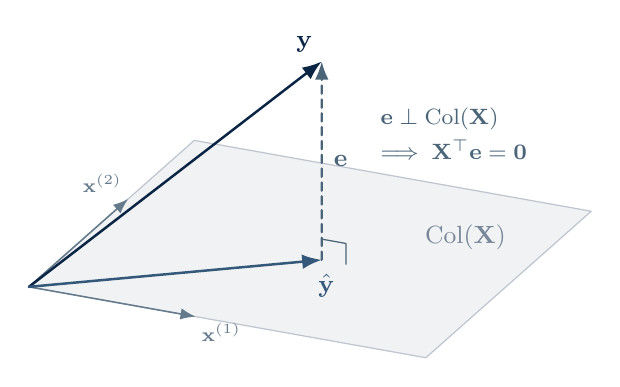
\begin{tikzpicture}[>=Latex,line cap=round,line join=round,scale=1.20]
  % ---- 平面 Col(X) ----
  \coordinate (O) at (0,0);
  \coordinate (U) at (4.20,-0.75);
  \coordinate (V) at (1.75,1.55);
  \fill[navy!6] (O) -- ($(O)+(U)$) -- ($(O)+(U)+(V)$) -- ($(O)+(V)$) -- cycle;
  \draw[navy!26,line width=0.45pt]
    (O) -- ($(O)+(U)$) -- ($(O)+(U)+(V)$) -- ($(O)+(V)$) -- cycle;

  % ---- 张成方向 ----
  \draw[->,steel!85,line width=0.55pt] (O) -- ($0.42*(U)$)
    node[below right,font=\scriptsize,inner sep=2pt]{$\bx^{(1)}$};
  \draw[->,steel!85,line width=0.55pt] (O) -- ($0.60*(V)$)
    node[above left,font=\scriptsize,inner sep=2pt]{$\bx^{(2)}$};

  % ---- 投影 ----
  \coordinate (P) at ($0.55*(U)+0.45*(V)$);
  \coordinate (Y) at ($(P)+(0,2.10)$);

  \draw[->,navy,line width=0.9pt] (O) -- (Y)
    node[above left,font=\small,inner sep=3pt]{$\by$};
  \draw[->,navy2,line width=0.9pt] (O) -- (P);
  \node[anchor=north,font=\small,inner sep=2pt,text=navy2] at ($(P)+(0.05,-0.09)$) {$\hat\by$};

  % 残差
  \draw[->,steel,line width=0.8pt,densely dashed] (P) -- (Y)
    node[midway,right,font=\small,inner sep=4pt]{$\be$};

  % 直角标记（沿平面方向）
  \draw[steel,line width=0.45pt]
    ($(P)+(0.256,-0.046)$) -- ($(P)+(0.256,0.174)$) -- ($(P)+(0,0.22)$);

  % 平面标签
  \node[navy!55,font=\small] at (4.62,0.52) {$\Col(\bX)$};

  % 右侧说明
  \node[anchor=west,font=\footnotesize,text=steel,align=left] at (3.62,1.62)
    {$\be\perp\Col(\bX)$\\[3pt]$\Longrightarrow\;\bX\tp\be=\bzero$};
\end{tikzpicture}

\caption{最小二乘的几何图像。所有可能的预测 $\bX\bw$ 铺成 $\R^N$ 中的一个平面 $\Col(\bX)$；$\hat\by$ 是 $\by$ 在该平面上的正交投影，残差 $\be$ 垂直于平面。}
\label{fig:projection}
\end{figure}

图 \ref{fig:projection} 把这个关系画了出来。由于投影由 $\by$ 唯一确定，可以把它写成一个线性算子：
\begin{equation}
  \hat\by=\bH\by,\qquad \bH=\bX(\bX\tp\bX)^{-1}\bX\tp .
  \label{eq:hat}
\end{equation}
$\bH$ 把观测 $\by$ 变成拟合值 $\hat\by$，像给 $\by$ 戴了顶帽子，故称\hl{帽子矩阵}。它的性质几乎都可以从「投影」二字读出来：

\begin{center}
\small
\begin{tabular}{@{}lll@{}}
\toprule
\rowcolor{navy!7}
\tabhead 性质 & \tabhead 式子 & \tabhead 解释\\
\midrule
对称 & $\bH\tp=\bH$ & 正交投影是自伴的\\
幂等 & $\bH^2=\bH$ & 投影两次等于投影一次\\
秩 & $\rank(\bH)=D$ & 投影的像就是 $\Col(\bX)$\\
迹 & $\tr(\bH)=D$ & 见下\\
残差算子 & $(\bI-\bH)^2=\bI-\bH$ & $\bI-\bH$ 也是投影，投向正交补\\
\bottomrule
\end{tabular}
\end{center}

其中 $\tr(\bH)=D$ 值得单独算一遍，因为它后面会变成「有效自由度」。利用迹的轮换性 $\tr(\bA\bB)=\tr(\bB\bA)$：
\begin{equation}
  \tr(\bH)=\tr\bigl(\bX(\bX\tp\bX)^{-1}\bX\tp\bigr)
  =\tr\bigl((\bX\tp\bX)^{-1}\bX\tp\bX\bigr)
  =\tr(\bI_D)=D .
\end{equation}

这句结论可以这样读：帽子矩阵的迹等于「模型实际用掉的参数个数」。第 4 节会看到，岭回归把 $\bH$ 换成 $\bH_\lambda$，迹就从 $D$ 连续地缩到 $0$——那正是「模型复杂度」的一个可计算的度量。

\marginnote{含截距且 $\by$ 中心化时 $R^2=\cos^2\theta$。}
还有一个小推论。若 $\by$ 已中心化、模型含截距，则 $\by$ 与残差正交，勾股定理给出
\begin{equation}
  \norm{\by}^2=\norm{\hat\by}^2+\norm{\be}^2 ,
\end{equation}
两边同除 $\norm{\by}^2$，得 $R^2=\norm{\hat\by}^2/\norm{\by}^2=\cos^2\theta$。所以 $R^2$ 的几何意义是「$\by$ 与它的投影之间夹角的余弦平方」——这也解释了为什么 $R^2$ 永远在 $[0,1]$ 内（含截距时）。

\subsection{秩、伪逆与最小范数解}

公式 \eqref{eq:ols} 里有个逆，而逆不一定存在。把情形分清楚：

\begin{center}
\small
\begin{tabular}{@{}llll@{}}
\toprule
\rowcolor{navy!7}
\tabhead 情形 & \tabhead 条件 & \tabhead $\bX\tp\bX$ & \tabhead 解\\
\midrule
列满秩 & $\rank(\bX)=D\le N$ & 可逆 & 唯一，$\hat\bw=(\bX\tp\bX)^{-1}\bX\tp\by$\\
行满秩 & $\rank(\bX)=N<D$ & 奇异 & 无穷多；最小范数解 $\bX\tp(\bX\bX\tp)^{-1}\by$\\
降秩 & $\rank(\bX)<\min(N,D)$ & 奇异 & 无穷多；用伪逆 $\bX^{+}\by$\\
\bottomrule
\end{tabular}
\end{center}

\begin{warn}[「无解」是个误称]
很多教材写「$\bX\tp\bX$ 不可逆，正规方程无法求解」，容易被读成「最小二乘问题无解」。这是不对的：正规方程\textbf{永远有解}。理由一行就够——$\bX\tp\by$ 属于 $\bX\tp$ 的列空间，而 $\mathrm{range}(\bX\tp)=\mathrm{range}(\bX\tp\bX)$，所以右端向量必定落在左端矩阵的值域里。

真正出问题的是\textbf{唯一性}：解有无穷多个，公式里的逆不存在只是这个事实的代数表现。
\end{warn}

多解时该选哪一个？注意所有最小二乘解给出\textbf{同一个}拟合值 $\hat\by$（它们投影到同一个点），训练误差完全一样——数据无法区分它们。既然无法区分，就选「最简单」的那个，即欧氏范数最小的：
\begin{equation}
  \hat\bw=\argmin_{\bw}\;\norm{\bw}_2
  \quad\text{s.t.}\quad \bw\in\argmin_{\bu}\norm{\bX\bu-\by}_2 .
  \label{eq:minnorm}
\end{equation}
这个选择不是随意的：第 4 节会看到，岭回归的解在 $\lambda\to0^{+}$ 时恰好收敛到 \eqref{eq:minnorm}。换句话说，最小范数解是「正则化强度趋于零」时的极限，而不是另一种人为约定。

一般情形用奇异值分解（SVD）最干净。设
\begin{equation}
  \bX=\bU\bSigma\bV\tp ,
\end{equation}
其中 $\bU\in\R^{N\times N}$、$\bV\in\R^{D\times D}$ 为正交阵，$\bSigma$ 为对角（含若干零）。把非零奇异值取倒数、零保持为零，得 $\bSigma^{+}$，则
\begin{equation}
  \bX^{+}=\bV\bSigma^{+}\bU\tp ,
  \qquad
  \hat\bw=\bX^{+}\by
  \label{eq:pinv}
\end{equation}
\emph{对任意} $\bX$（无论秩亏与否）都给出最小范数最小二乘解。这就是伪逆（Moore--Penrose 广义逆）的全部内容。

\begin{add}[为什么最小范数解「最合理」]
把解集写出来会更清楚。若 $\bw_0$ 是一个最小二乘解，则全部解构成仿射集 $\bw_0+\ker(\bX)$：加上任何落在零空间里的方向，拟合值 $\bX\bw$ 都不变。于是「选哪个」等价于「在解集这个仿射子空间里找离原点最近的点」，而最近点就是 $\bw_0$ 在 $\ker(\bX)$ 的正交补上的投影——它唯一，且垂直于零空间。

这也解释了为什么列相关的特征会让系数「乱跳」：把 $w_1$ 加大、$w_2$ 相应减小，只要方向落在零空间里，预测就完全不变。系数不可辨识，但预测可辨识。
\end{add}

\subsection{数值实现：公式不等于算法}

教科书停在 \eqref{eq:ols}，工程上却不能照着写。原因有两个：复杂度，与数值稳定性。

\subsubsection{复杂度}

\begin{center}
\small
\begin{tabular}{@{}llll@{}}
\toprule
\rowcolor{navy!7}
\tabhead 方法 & \tabhead 主要步骤 & \tabhead 复杂度 & \tabhead 稳定性由什么决定\\
\midrule
正规方程 + Cholesky & 组装 $\bX\tp\bX$，再分解 & $\sim ND^2+D^3/3$ & $\kappa(\bX)^2$\\
QR 分解 & $\bX=\bQ\bR$，解 $\bR\bw=\bQ\tp\by$ & $\sim 2ND^2$ & $\kappa(\bX)$\\
SVD & $\bX=\bU\bSigma\bV\tp$，用伪逆 & $\sim 2ND^2$（常数更大） & $\kappa(\bX)$，可处理秩亏\\
\bottomrule
\end{tabular}
\end{center}

三者的量级都是 $O(ND^2)$，在 $N\gg D$ 时差别不大。真正拉开差距的是第二列。

\subsubsection{条件数被平方}

矩阵的条件数 $\kappa(\bX)=\sigma_{\max}/\sigma_{\min}$ 衡量「输入的小扰动会被放大多少倍」。正规方程把这件事弄坏了，因为
\begin{equation}
  \kappa(\bX\tp\bX)=\frac{\sigma_{\max}^2}{\sigma_{\min}^2}=\kappa(\bX)^2 .
\end{equation}
若 $\kappa(\bX)=10^{3}$，则 $\kappa(\bX\tp\bX)=10^{6}$。双精度浮点约有 $16$ 位十进制有效数字，解正规方程会白白损失 $6$ 位。$\kappa(\bX)=10^{8}$ 时，$\bX\tp\bX$ 在计算机里可能已经「不可逆」了——不是因为数学上奇异，而是因为 $\sigma_{\min}^2$ 被舍入吃掉了。

\begin{keybox}[实践建议]
\begin{enumerate}[label=(\arabic*),leftmargin=1.9em]
  \item \textbf{不要显式求逆。}$(\bX\tp\bX)^{-1}$ 只应出现在公式里；代码里应当「解方程组」，而不是「先求逆再相乘」。
  \item \textbf{默认用 SVD 或 QR。}\texttt{numpy.linalg.lstsq} 默认走 SVD；\texttt{scipy.linalg.lstsq} 可选 \texttt{lapack\_driver='gelsd'}（SVD）或 \texttt{'gelsy'}（QR）。
  \item \textbf{特征共线时先想办法。}标准化、删冗余列、加岭项（\S4.2，$\lambda$ 会把条件数压成 $(\sigma_{\max}^2+\lambda)/(\sigma_{\min}^2+\lambda)$），都比硬解正规方程稳妥。
\end{enumerate}
\end{keybox}

% ============================================================
%  第 3 节  概率视角
% ============================================================

\section{概率视角：MLE 与 MAP}

第 2 节把平方损失当成一个「合理的选择」。这一节要说明，它其实是一个\textbf{假设的推论}：只要假定噪声服从高斯分布，最小二乘就恰好是极大似然估计。再往前一步，给参数加一个先验，正则项就自然出现了。

\subsection{高斯噪声下的极大似然}

设观测由「真实函数 + 噪声」生成：
\begin{equation}
  y_i=\bw\tp\bx_i+\epsilon_i,\qquad
  \epsilon_1,\dots,\epsilon_N\;\overset{\text{i.i.d.}}{\sim}\;\mathcal N(0,\sigma^2).
  \label{eq:noisemodel}
\end{equation}
「独立同分布」四个字承载了两条假设：样本之间互不影响；每个样本的噪声来自同一个分布。于是
\begin{equation}
  y_i\mid\bx_i\;\sim\;\mathcal N(\bw\tp\bx_i,\;\sigma^2),
\end{equation}
且给定 $\bX$ 后各 $y_i$ 条件独立。

似然函数是「把观测到的 $\by$ 当作 $\bw$ 的函数」：
\begin{equation}
  p(\by\mid\bX,\bw)=\prod_{i=1}^{N}\frac{1}{\sqrt{2\pi}\,\sigma}
  \exp\!\left(-\frac{(y_i-\bw\tp\bx_i)^2}{2\sigma^2}\right).
\end{equation}
连乘不好处理，取对数把它变成求和：
\begin{align}
  \ell(\bw)=\log p(\by\mid\bX,\bw)
  &=-\frac{N}{2}\log(2\pi\sigma^2)-\frac{1}{2\sigma^2}\sum_{i=1}^{N}(y_i-\bw\tp\bx_i)^2 .
  \label{eq:loglik}
\end{align}

现在看 \eqref{eq:loglik} 的结构：第一项与 $\bw$ 无关，第二项是残差平方和乘上一个负常数。于是
\begin{equation}
  \argmax_{\bw}\ell(\bw)
  =\argmax_{\bw}\left[-\frac{1}{2\sigma^2}\sum_i(y_i-\bw\tp\bx_i)^2\right]
  =\argmin_{\bw}\sum_i(y_i-\bw\tp\bx_i)^2 .
  \label{eq:mle}
\end{equation}

\begin{keybox}[结论]
在高斯噪声假设下，\textbf{极大似然估计与最小二乘估计是同一个估计}。$\sigma^2$ 的具体取值不影响 $\hat\bw$——它只是一个缩放因子，而最大化一个负的平方和不依赖于缩放多少。
\end{keybox}

顺便把 $\sigma^2$ 也估出来。对 \eqref{eq:loglik} 关于 $\sigma^2$ 求导并令其为零，得
\begin{equation}
  \hat\sigma^2_{\text{MLE}}=\frac{1}{N}\sum_{i=1}^{N}\hat e_i^2 .
\end{equation}
这个估计是\hl{有偏}的：分母是 $N$ 而不是 $N-D$。原因不神秘——残差 $\hat e_i$ 不是独立信息，它们被 $D$ 个正规方程约束住了（等价地，$\hat\by$ 落在 $D$ 维子空间里，只剩 $N-D$ 维自由度）。无偏估计是
\begin{equation}
  \hat\sigma^2=\frac{1}{N-D}\sum_{i=1}^{N}\hat e_i^2 ,
  \label{eq:sigmahat}
\end{equation}
它后面会出现在系数的标准误里（\S5.3）。对本讲例题，$\hat\sigma^2=34.07/(8-2)=5.68$，$\hat\sigma=2.38$ 分。

\begin{add}[这条等价关系的反面更有用]
既然「平方损失 $\Leftrightarrow$ 高斯噪声」，那么噪声不是高斯时，平方损失就不再是 MLE。若噪声服从拉普拉斯分布（尖峰厚尾），对应的 MLE 是最小化残差绝对值之和：
\begin{equation}
  \hat\bw_{\text{LAD}}=\argmin_{\bw}\sum_{i=1}^{N}\abs{y_i-\bw\tp\bx_i} ,
\end{equation}
称为\hl{最小绝对偏差}回归。它估计的是条件中位数而非条件均值，对离群点稳健得多。

所以「为什么用平方损失」这个问题的完整答案是：\emph{因为你默认了高斯噪声}。这个默认在多数场合够用，但你应当知道它何时失效。
\end{add}

\subsection{高斯先验下的 MAP：岭回归登场}

极大似然只用了数据。若我们对 $\bw$ 事先有看法——比如「系数大概不会太离谱」——就该把它写进先验，改用最大后验估计。由贝叶斯公式，
\begin{equation}
  p(\bw\mid\by)\;\propto\;p(\by\mid\bw)\,p(\bw),
\end{equation}
取负对数后，「最大化后验」变成「最小化负对数后验」：
\begin{equation}
  \hat\bw_{\text{MAP}}
  =\argmin_{\bw}\bigl[-\log p(\by\mid\bw)-\log p(\bw)\bigr].
\end{equation}

取零均值、各分量独立同方差的高斯先验
\begin{equation}
  \bw\sim\mathcal N(\bzero,\sigma_0^2\bI),
  \qquad
  -\log p(\bw)=\frac{1}{2\sigma_0^2}\norm{\bw}_2^2+\text{const}.
\end{equation}
代回目标函数（常数略去）：
\begin{equation}
  \frac{1}{2\sigma^2}\norm{\by-\bX\bw}_2^2+\frac{1}{2\sigma_0^2}\norm{\bw}_2^2 .
\end{equation}
两边同乘 $2\sigma^2$（不改变最优点），得到
\begin{equation}
  \hat\bw_{\text{MAP}}
  =\argmin_{\bw}\Bigl[\;\norm{\by-\bX\bw}_2^2+\underbrace{\frac{\sigma^2}{\sigma_0^2}}_{\lambda}\norm{\bw}_2^2\;\Bigr].
  \label{eq:ridgemap}
\end{equation}

这正是岭回归的目标函数，正则化强度由噪声方差与先验方差之比决定：
\begin{equation}
  \boxed{\;\lambda=\frac{\sigma^2}{\sigma_0^2}\;}
  \label{eq:lambda}
\end{equation}

\begin{center}
\small
\begin{tabular}{@{}lll@{}}
\toprule
\rowcolor{navy!7}
\tabhead 情形 & \tabhead $\lambda$ & \tabhead 直觉\\
\midrule
噪声很大（$\sigma^2\uparrow$） & 变大 & 数据不可信，多听先验的\\
先验很宽（$\sigma_0^2\uparrow$） & 变小 & 对 $\bw$ 没什么主见，多听数据的\\
先验很窄（$\sigma_0^2\to0$） & $\to\infty$ & 坚信 $\bw=\bzero$，无视数据\\
\bottomrule
\end{tabular}
\end{center}

这张表说明了一件常被忽略的事：$\lambda$ 不是「玄学超参数」，它有明确的统计含义，是「数据的不确定性」与「先验的确定性」的比值。实践中用交叉验证选 $\lambda$（\S5.5），本质上是在从数据里估这个比值。

\begin{warn}[MAP 不是贝叶斯推断]
最大后验只取后验分布的\emph{众数}，仍然是一个点估计。完整的贝叶斯做法要对后验积分（预测分布 $p(y_*\mid\bx_*)=\int p(y_*\mid\bx_*,\bw)p(\bw\mid\by)\dd\bw$），得到的不只是点，还有不确定性。在共轭高斯设定下这个积分有闭式解，那就是\hl{贝叶斯线性回归}——它给出的预测方差会随 $\bx_*$ 远离训练数据而增大，这是点估计做不到的。
\end{warn}

\subsection{拉普拉斯先验下的 MAP：Lasso}

把先验换成拉普拉斯分布。它的密度在零点有一个尖峰：
\begin{equation}
  p(w_j)=\frac{1}{2b}\exp\!\left(-\frac{\abs{w_j}}{b}\right),
  \qquad
  -\log p(\bw)=\frac{1}{b}\norm{\bw}_1+\text{const}.
\end{equation}
同样的流程：负对数后验为 $\frac{1}{2\sigma^2}\text{RSS}+\frac{1}{b}\norm{\bw}_1$，两边乘 $2\sigma^2$：
\begin{equation}
  \hat\bw_{\text{MAP}}
  =\argmin_{\bw}\Bigl[\;\norm{\by-\bX\bw}_2^2
  +\underbrace{\frac{2\sigma^2}{b}}_{\lambda}\norm{\bw}_1\;\Bigr].
  \label{eq:lassomap}
\end{equation}

\begin{keybox}[对称的美感]
\begin{itemize}
  \item 噪声分布决定\hl{损失函数}：高斯 $\to$ 平方和；拉普拉斯 $\to$ 绝对值和。
  \item 参数先验决定\hl{正则项}：高斯 $\to$ $L_2$；拉普拉斯 $\to$ $L_1$。
\end{itemize}
两件事各管一头，可以自由组合。这是第 4 节全部内容的骨架。
\end{keybox}

\subsection{两张对照表}

\begin{table}[htbp]
\centering
\small
\caption{三种估计的假设与结果}
\label{tab:three}
\begin{tabular}{@{}llll@{}}
\toprule
\rowcolor{navy!7}
\tabhead 估计 & \tabhead 假设 & \tabhead 目标函数 & \tabhead 解的性质\\
\midrule
最小二乘 / MLE & 高斯噪声 & $\norm{\by-\bX\bw}^2$ & 闭式解，无偏\\
岭回归 / MAP & 高斯噪声 + 高斯先验 & $\norm{\by-\bX\bw}^2+\lambda\norm{\bw}_2^2$ & 闭式解，有偏收缩\\
Lasso / MAP & 高斯噪声 + 拉普拉斯先验 & $\norm{\by-\bX\bw}^2+\lambda\norm{\bw}_1$ & 无闭式解，稀疏\\
\bottomrule
\end{tabular}
\end{table}

\begin{table}[htbp]
\centering
\small
\caption{噪声模型与先验模型的组合}
\label{tab:combo}
\begin{tabular}{@{}lccc@{}}
\toprule
\rowcolor{navy!7}
\tabhead & \tabhead 无先验（MLE） & \tabhead 高斯先验 & \tabhead 拉普拉斯先验\\
\midrule
高斯噪声 & 最小二乘（$L_2$ 损失） & 岭回归 & Lasso\\
拉普拉斯噪声 & LAD（$L_1$ 损失） & 近似 Huber & 罕用\\
\bottomrule
\end{tabular}
\end{table}

表 \ref{tab:combo} 值得多看一会儿，因为它把两个极易混淆的概念分开了：

\begin{itemize}
  \item \textbf{$L_1$ 损失}（左列第二行）：惩罚的是\emph{残差}，用来对付离群点，估计条件中位数。
  \item \textbf{$L_1$ 正则}（右列第一行）：惩罚的是\emph{参数}，用来对付过拟合，产生稀疏解。
\end{itemize}

两者形式上都带绝对值，作用对象完全不同。笔记里特意提醒过这一点，此处用一个 $2\times2$ 表把它钉死：\emph{先验管参数，噪声管残差}。

\subsection{补充：为什么拉普拉斯先验偏爱零}

高斯密度在零点光滑、导数为零，像一个圆润的小山包；拉普拉斯密度在零点有尖角，导数从 $-1/b$ 跳到 $+1/b$。这个差别在优化时会被放大：

对于高斯先验，把某个系数从 $0$ 推到 $\delta$，负对数先验只增加 $O(\delta^2)$——一阶几乎免费。对于拉普拉斯先验，增加的是 $O(\delta)$——有固定的「起步价」。

于是只要数据对某个系数的支持不够强（梯度推力小于这个起步价），最优选择就是让它\textbf{精确等于零}，而不是「小一点」。这就是稀疏性的来源。第 4 节会把这个直觉写成次梯度条件。

% ============================================================
%  第 4 节  正则化
% ============================================================

\section{正则化}

\subsection{过拟合是怎样发生的}

先把两个误差分清楚。\hl{训练误差}是模型在已经见过的数据上的平均损失；\hl{泛化误差}是它在同分布的新样本上的期望损失。我们真正关心的是后者，但只能观测到前者。

两者可以差得很远，而且差距随模型复杂度单调扩大。线性回归里有一个干净的例子说明这一点：

\begin{prop}[$N<D$ 时训练误差可以为零]
设 $\bX\in\R^{N\times D}$ 行满秩且 $N<D$。则方程 $\bX\bw=\by$ 有解，即存在 $\bw$ 使训练误差恰好为零。
\end{prop}

\begin{proof}
$\bX$ 行满秩意味着 $\rank(\bX)=N$，即 $\bX$ 的列空间是整个 $\R^N$。既然 $\by\in\R^N=\Col(\bX)$，它就一定能写成列的线性组合，即存在 $\bw$ 使 $\bX\bw=\by$。这样的 $\bw$ 有无穷多个（零空间维数为 $D-N>0$）。
\end{proof}

这个结论很刺眼：只要特征比样本多，模型就能把训练集\emph{背}下来，训练误差为零，但对新样本毫无保证。它记住的是噪声，不是规律。

\begin{add}[为什么「参数多」必然带来风险]
从自由度看最清楚。$N$ 个观测提供了 $N$ 条独立信息；模型有 $D$ 个自由参数。当 $D$ 逼近 $N$，模型有足够的自由度去迁就每一个观测的随机波动。第 \S2.5 节已经看到，此时解甚至不唯一——数据本身无法确定参数。

反过来，若 $D\ll N$，模型只能捕捉数据中「最主流的」那个方向，随机波动被平均掉，泛化反而稳。
\end{add}

应对过拟合有三条路：
\begin{enumerate}[label=(\arabic*)]
  \item \textbf{加数据}：最根本，但往往做不到或太贵；
  \item \textbf{降维}：减特征（PCA、特征选择），直接减少 $D$；
  \item \textbf{正则化}：不减特征，而是限制参数的\emph{大小}，等价于缩小假设空间。
\end{enumerate}
本讲只讲第三条，但请记住它是三条里最「便宜」的一条，因此也是最常被滥用的。

\subsection{岭回归：把参数往原点拉}

\subsubsection{闭式解}

在平方损失上加一个二次惩罚：
\begin{equation}
  L_\lambda(\bw)=\norm{\by-\bX\bw}_2^2+\lambda\norm{\bw}_2^2,\qquad \lambda>0 .
  \label{eq:ridgeobj}
\end{equation}
求梯度（第一项见 \eqref{eq:grad}，第二项是 $\lambda\norm{\bw}^2$，梯度 $2\lambda\bw$）：
\begin{equation}
  \nabla L_\lambda=2\bX\tp(\bX\bw-\by)+2\lambda\bw .
\end{equation}
令其为零：
\begin{equation}
  (\bX\tp\bX+\lambda\bI)\hat\bw_\lambda=\bX\tp\by
  \quad\Longrightarrow\quad
  \boxed{\;\hat\bw_\lambda=(\bX\tp\bX+\lambda\bI)^{-1}\bX\tp\by\;}
  \label{eq:ridge}
\end{equation}

\begin{prop}[岭回归总有唯一解]
若 $\lambda>0$，则 $\bX\tp\bX+\lambda\bI$ 正定，因而对任意 $\bX$（包括秩亏的情形）都可逆。
\end{prop}
\begin{proof}
设 $\bu\ne\bzero$，则 $\bu\tp(\bX\tp\bX+\lambda\bI)\bu=\norm{\bX\bu}_2^2+\lambda\norm{\bu}_2^2\ge\lambda\norm{\bu}^2>0$。正定故可逆。
\end{proof}

这条副产品值得强调：\textbf{岭回归顺带解决了秩亏问题}。哪怕特征完全共线、$\bX\tp\bX$ 奇异，只要加一个 $\lambda>0$，就能解出唯一的 $\hat\bw_\lambda$。而且当 $\lambda\to0^+$ 时，这个解连续地收敛到 \S2.5 的最小范数解。

顺带说明：\eqref{eq:ridge} 与第 3 节的 MAP 解 \eqref{eq:ridgemap} 是同一个式子，只是走到它的路径不同——那里从「先验 + 似然」出发，这里从「损失 + 惩罚」出发。$\lambda=\sigma^2/\sigma_0^2$ 就是两条路的接头：它把「先验有多确定」翻译成「惩罚有多重」。

\subsubsection{SVD 视角：每个方向被收缩多少}

把 $\bX=\bU\bSigma\bV\tp$ 代入 \eqref{eq:ridge}：
\begin{align}
  \hat\bw_\lambda
  &=\bigl(\bV\bSigma^2\bV\tp+\lambda\bI\bigr)^{-1}\bV\bSigma\bU\tp\by
  =\bV(\bSigma^2+\lambda\bI)^{-1}\bSigma\bU\tp\by \notag\\
  &=\sum_{j=1}^{r}\frac{d_j}{d_j^2+\lambda}\bigl(\bu_j\tp\by\bigr)\bv_j
  \;=\;\sum_{j=1}^{r}\underbrace{\frac{d_j^2}{d_j^2+\lambda}}_{\text{收缩因子}}\cdot
  \frac{1}{d_j}\,\bu_j\tp\by\;\bv_j .
  \label{eq:ridgesvd}
\end{align}
对比最小二乘解 $\hat\bw_{\text{OLS}}=\sum_j \frac{1}{d_j}(\bu_j\tp\by)\bv_j$，可以看到：\hl{岭回归没有改变方向，只是把每个方向上的系数乘了一个小于 1 的因子。}

\begin{itemize}
  \item $d_j$ 很大（数据在这个方向上信息充足）：$d_j^2/(d_j^2+\lambda)\approx1$，几乎不动；
  \item $d_j$ 很小（这个方向几乎无法从数据中辨识）：因子 $\approx d_j^2/\lambda\approx0$，被狠狠压向零。
\end{itemize}

\begin{figure}[htbp]
\centering
% ---- 插图：fig-shrink ----
% 四张图：收缩、软阈值、L1-L2、偏差方差
\begin{tikzpicture}
\begin{axis}[
  width=10.2cm,height=6.0cm,
  xlabel={奇异值 $d$},
  ylabel={保留比例},
  xmin=0,xmax=8,ymin=0,ymax=1.02,
  axis lines=left,
  every axis plot/.append style={line width=0.9pt},
  label style={font=\footnotesize,color=steel},
  tick label style={font=\scriptsize,color=steel},
  xtick={0,2,4,6,8},ytick={0,0.25,0.5,0.75,1},
  yticklabel style={/pgf/number format/fixed,/pgf/number format/precision=2},
  legend style={font=\scriptsize,draw=navy!25,fill=white,fill opacity=0.9,
    text opacity=1,at={(0.985,0.14)},anchor=east},
  grid=major,grid style={navy!7},
]
\addplot[domain=0:8,samples=140,navy] {x^2/(x^2+0.5)};
\addlegendentry{$\lambda=0.5$}
\addplot[domain=0:8,samples=140,navy2,dashed] {x^2/(x^2+4)};
\addlegendentry{$\lambda=4$}
\addplot[domain=0:8,samples=140,steel,densely dotted] {x^2/(x^2+16)};
\addlegendentry{$\lambda=16$}
\end{axis}
\end{tikzpicture}

\caption{岭回归的收缩效应。横轴是某个方向上的奇异值，纵轴是该方向保留下来的系数比例。奇异值小的方向（数据几乎无法辨识的方向）被强烈压缩；奇异值大的方向几乎不受影响。$\lambda$ 越大，整条曲线越靠右，收缩越强。}
\label{fig:shrink}
\end{figure}

图 \ref{fig:shrink} 是理解岭回归的关键。它解释了为什么岭回归「稳」：\textbf{方差大的方向恰恰是 $\bX\tp\bX$ 小特征值对应的方向}，岭回归选择性地压掉了这些方向，用一点偏差换来了方差的显著下降。这正是偏差—方差权衡的一个具体实现。

\subsubsection{有效自由度}

把帽子矩阵换成岭回归的版本：
\begin{equation}
  \bH_\lambda=\bX(\bX\tp\bX+\lambda\bI)^{-1}\bX\tp
  =\bU\,\mathrm{diag}\!\left(\frac{d_j^2}{d_j^2+\lambda}\right)\bU\tp .
\end{equation}
它的迹给出一个连续变化的「有效参数个数」：
\begin{equation}
  \mathrm{df}(\lambda)=\tr(\bH_\lambda)=\sum_{j=1}^{r}\frac{d_j^2}{d_j^2+\lambda}\;\in\;(0,\,D] .
  \label{eq:edf}
\end{equation}
$\lambda=0$ 时 $\mathrm{df}=D$，就是普通最小二乘；$\lambda\to\infty$ 时 $\mathrm{df}\to0$，模型退化为常数。中间的值可以理解为「模型实际用掉了几个参数」。

\begin{add}[有效自由度的用处]
它把「$\lambda$ 越大模型越简单」这句定性的话变成了一个可计算的量。给定数据，你可以先画出 $\mathrm{df}(\lambda)$ 曲线，看 $\lambda$ 取多大时模型的有效复杂度降到期望水平，再去交叉验证微调。

注意 $\mathrm{df}(\lambda)$ 随 $\lambda$ 单调下降（每一项都是 $\lambda$ 的减函数），所以「更简单的模型」这件事有严格定义，不依赖直觉。
\end{add}

\subsubsection{几何图像}

\eqref{eq:ridgeobj} 与下面这个带约束的问题是等价的（拉格朗日乘子，$\lambda$ 与 $C$ 一一对应）：
\begin{equation}
  \min_{\bw}\;\norm{\by-\bX\bw}^2
  \quad\text{s.t.}\quad \norm{\bw}_2\le C .
  \label{eq:ridgecon}
\end{equation}
损失函数的等值线是椭圆（因为 $\bX\tp\bX$ 一般不是单位阵，椭圆会被拉长、旋转），约束区域是一个球。两者相切之处就是解。二维时球是圆，切点通常落在圆周上的任意位置——\textbf{两个坐标一般都不为零}。所以在二维图景里，岭回归不产生稀疏解。图 \ref{fig:l1l2}(b) 会把这两个约束区域并排画出来。

\subsection{Lasso：把参数压到零}

\subsubsection{目标与最优性条件}

\begin{equation}
  L^{\text{L}}_\lambda(\bw)=\norm{\by-\bX\bw}_2^2+\lambda\norm{\bw}_1
  =\norm{\by-\bX\bw}_2^2+\lambda\sum_{j=1}^{D}\abs{w_j} .
  \label{eq:lassoobj}
\end{equation}
绝对值在 $w_j=0$ 处不可导，于是「梯度为零」要换成「零属于次微分」。记残差 $\mathbf r=\by-\bX\bw$，则

\begin{center}
\small
\begin{tabular}{@{}ll@{}}
\toprule
\rowcolor{navy!7}
\tabhead 情形 & \tabhead 最优性条件\\
\midrule
$w_j\neq0$ & $-2(\bX\tp\mathbf r)_j+\lambda\,\sign(w_j)=0$\\[2pt]
$w_j=0$   & $\abs{2(\bX\tp\mathbf r)_j}\le\lambda$\\
\bottomrule
\end{tabular}
\end{center}

换个说法会更直观。令 $c_j=(\bX\tp\mathbf r)_j$，它是「第 $j$ 个特征与当前残差的内积」，可以读作两者尚未解释的相关性。条件变成
\begin{equation}
  c_j=\frac{\lambda}{2}\sign(w_j)\ \ (w_j\ne0),
  \qquad
  \abs{c_j}\le\frac{\lambda}{2}\ \ (w_j=0).
\end{equation}

\begin{keybox}[Lasso 在做什么]
在所有被\textbf{选入}的特征上，它与残差的相关性被钉在同一个水平 $\lambda/2$ 上；相关系数低于这个阈值的特征，一律被压到零并留在零。所以 $\lambda$ 直接控制「进入模型的门槛」。
\end{keybox}

\subsubsection{正交设计下的闭式解：软阈值}

一般情形下 Lasso 没有闭式解，但有一个特例能看清机制。若 $\bX\tp\bX=\bI$（特征正交且已归一），记 $\bz=\bX\tp\by$，则 $c_j=z_j-w_j$，条件变为
\begin{equation}
  2(z_j-w_j)=\lambda\,\sign(w_j)\ \ \text{或}\ \ w_j=0 .
\end{equation}
逐坐标解出：
\begin{equation}
  \boxed{\;\hat w_j=\sign(z_j)\max\!\Bigl(\abs{z_j}-\frac{\lambda}{2},\,0\Bigr)\;}
  \label{eq:soft}
\end{equation}

这就是\hl{软阈值}算子。它把每个坐标朝零的方向平移 $\lambda/2$，平移量不够就归零。

\begin{figure}[htbp]
\centering
% ---- 插图：fig-soft ----
\begin{tikzpicture}[x=1.12cm,y=1.00cm,>=Latex,line cap=round]
  % 坐标轴
  \draw[->,navy!45,line width=0.5pt] (-3.55,0) -- (3.80,0)
    node[below,font=\footnotesize,inner sep=2pt]{$z_j$};
  \draw[->,navy!45,line width=0.5pt] (0,-3.55) -- (0,3.80)
    node[left,font=\footnotesize,inner sep=2pt]{$\hat w_j$};

  % 刻度（只标阈值）
  \foreach \t in {-3,-2,2,3}{
    \draw[navy!40,line width=0.4pt] (\t,0.08) -- (\t,-0.08);
    \draw[navy!40,line width=0.4pt] (0.08,\t) -- (-0.08,\t);
  }
  \draw[navy!60,line width=0.5pt] (-1,0.10) -- (-1,-0.10);
  \draw[navy!60,line width=0.5pt] (1,0.10) -- (1,-0.10);
  \node[font=\scriptsize,color=navy,below=2pt] at (-1,0) {$-\tfrac{\lambda}{2}$};
  \node[font=\scriptsize,color=navy,below=2pt] at (1,0) {$\tfrac{\lambda}{2}$};

  % 对角线
  \draw[steel,densely dashed,line width=0.6pt] (-3.35,-3.35) -- (3.35,3.35);
  \node[font=\footnotesize,color=steel,anchor=west,inner sep=2pt] at (2.42,2.72) {$\hat w=z$};

  % 死区
  \draw[navy!35,densely dotted,line width=0.6pt] (-1,-3.4) -- (-1,3.4);
  \draw[navy!35,densely dotted,line width=0.6pt] (1,-3.4) -- (1,3.4);

  % 软阈值曲线（先描白边，避免与横轴重叠）
  \draw[white,line width=4pt] (-3.4,-2.4) -- (-1,0) -- (1,0) -- (3.4,2.4);
  \draw[navy,line width=1.2pt] (-3.4,-2.4) -- (-1,0) -- (1,0) -- (3.4,2.4);

  % 标注
  \node[font=\footnotesize,color=navy,anchor=east] (dz) at (-0.22,0.70) {死区};
  \draw[->,navy!60,line width=0.45pt] (dz.south east) -- (-0.10,0.12);
\end{tikzpicture}

\caption{软阈值（$\lambda=2$，故阈值为 $\lambda/2=1$）。虚线是对角线 $\hat w=z$，实线是 Lasso 的解。$\abs{z_j}\le1$ 的坐标被压成精确的零，这是稀疏性的直接来源。}
\label{fig:soft}
\end{figure}

图 \ref{fig:soft} 把 \eqref{eq:soft} 画了出来。中间那段平坦的「死区」就是稀疏的产地：只要原始估计 $\abs{z_j}$ 落在阈值内，输出就是零。也请注意这条曲线的形状——它连续，但有一个折点；相比之下，硬阈值（直接截断）是不连续的，这会让估计的方差更大。

\subsubsection{为什么 \texorpdfstring{$L_1$}{L1} 能产生稀疏解}

三条理由，从严格到直观。

\paragraph{其一，推力不随参数衰减}
对 $L_2$ 项求导得 $2\lambda w_j$：当 $w_j\to0$ 时，把它继续往零推的力也趋于零，于是它只能无限接近零，永远到不了。对 $L_1$ 项，次梯度的模长恒为 $\lambda$，与 $w_j$ 的大小无关——只要还在动，力就是满的，所以能一口气推到零并停住。

\paragraph{其二，零点的次微分包含原点}
$L_1$ 在 $0$ 处的次微分是区间 $[-\lambda,\lambda]$，不是单点。这意味着只要数据给出的梯度落在区间内，$w_j=0$ 就满足最优性条件。$L_2$ 在 $0$ 处的次微分只有单点 $\{0\}$，要求苛刻得多。

\paragraph{其三，几何上更容易切到顶点}
损失等高线是椭圆，约束区域是 $\norm{\bw}_1\le C$ 的菱形。菱形有顶点落在坐标轴上，而顶点处更「尖」，切点落在顶点的可能性比落在边上大。

\begin{figure}[htbp]
\centering
% ---- 插图：fig-l1l2 ----
\begin{tikzpicture}[x=1.62cm,y=1.62cm,>=Latex,line cap=round]
% ================= 左：L1 =================
\begin{scope}
  \fill[navy!8] (1,0) -- (0,1) -- (-1,0) -- (0,-1) -- cycle;
  \draw[navy!50,line width=0.55pt] (1,0) -- (0,1) -- (-1,0) -- (0,-1) -- cycle;
  \draw[navy,line width=0.8pt,domain=0:360,samples=180]
    plot ({1.323+0.2687*cos(\x)+0.5374*sin(\x)},
          {0.211+0.2687*cos(\x)-0.5374*sin(\x)});
  % OLS 中心
  \draw[navy,line width=0.7pt] (1.323,0.211) +(0.075,0) -- +(-0.075,0)
    (1.323,0.211) +(0,0.075) -- +(0,-0.075);
  % 切点
  \fill[gold] (1,0) circle (1.9pt);
  \draw[gold!70,line width=0.4pt] (1,0) circle (3.4pt);
  % 标注
  \draw[->,gold,line width=0.5pt] (0.86,-1.06) -- (0.99,-0.12);
  \node[font=\footnotesize\bfseries,color=gold,anchor=north,inner sep=1pt] at (0.86,-1.12) {$\hat w_2=0$};
  % 坐标轴
  \draw[->,steel!60,line width=0.4pt] (-1.22,0) -- (2.58,0) node[below,font=\tiny,inner sep=1pt]{$w_1$};
  \draw[->,steel!60,line width=0.4pt] (0,-1.45) -- (0,1.40) node[left,font=\tiny,inner sep=1pt]{$w_2$};
\end{scope}

% ================= 右：L2 =================
\begin{scope}[xshift=7.10cm]
  \fill[navy!8] (0,0) circle (0.848);
  \draw[navy!50,line width=0.55pt] (0,0) circle (0.848);
  \draw[navy,line width=0.8pt,domain=0:360,samples=180]
    plot ({1.323+0.2687*cos(\x)+0.5374*sin(\x)},
          {0.211+0.2687*cos(\x)-0.5374*sin(\x)});
  \draw[navy,line width=0.7pt] (1.323,0.211) +(0.075,0) -- +(-0.075,0)
    (1.323,0.211) +(0,0.075) -- +(0,-0.075);
  % 切点
  \fill[gold] (0.779,0.335) circle (1.9pt);
  \draw[gold!70,line width=0.4pt] (0.779,0.335) circle (3.4pt);
  % 标注
  \draw[->,gold,line width=0.5pt] (0.60,-1.06) -- (0.77,0.26);
  \node[font=\footnotesize\bfseries,color=gold,anchor=north,inner sep=1pt] at (0.60,-1.12) {两个都非零};
  % 坐标轴
  \draw[->,steel!60,line width=0.4pt] (-1.10,0) -- (2.58,0) node[below,font=\tiny,inner sep=1pt]{$w_1$};
  \draw[->,steel!60,line width=0.4pt] (0,-1.45) -- (0,1.40) node[left,font=\tiny,inner sep=1pt]{$w_2$};
\end{scope}
\end{tikzpicture}

\caption{$L_1$ 与 $L_2$ 约束的几何对比（权重空间的二维截面）。椭圆是损失函数的等值线，十字标出普通最小二乘解 $\hat\bw_{\text{OLS}}$，圆点是切点。\textbf{左}：菱形 $\norm{\bw}_1\le C$ 与椭圆相切于\emph{顶点} $(1,0)$，故 $\hat w_2=0$，解是稀疏的。\textbf{右}：圆 $\norm{\bw}_2\le C$ 与椭圆相切于一般位置，两个分量都不为零。两图取自同一组 $\bX\tp\bX$ 与同一个 $\hat\bw_{\text{OLS}}$，因此差异完全由约束区域的形状造成。}
\label{fig:l1l2}
\end{figure}

\begin{warn}[几何论证只是直觉，不是证明]
图 \ref{fig:l1l2} 是二维示意图。它告诉你「为什么可能稀疏」，但没有证明「一定稀疏」或「稀疏多少」：高维情形无法用平面图代替，切点是否落在顶点还取决于 $\bX\tp\bX$ 的具体结构。

严格的结论来自次梯度分析（即上面的「其二」），或者 KKT 条件。把几何图当作记忆的钩子可以，当作论证不行。
\end{warn}

\subsubsection{实践中的几个坑}

\begin{enumerate}[label=(\arabic*)]
  \item \textbf{相关特征之间的选择不稳定。}若两个特征高度相关、信息几乎重复，Lasso 往往只保留其中一个，但保留谁带有随机性——换一份样本，可能换成另一个。若你关心「哪一组特征重要」而不是「哪一个」，请用 Elastic Net 或 group Lasso。
  \item \textbf{$N<D$ 时的上限。}可以证明（一般位置下），Lasso 至多选出 $N$ 个非零系数。所以从一万个特征里选一千个、而样本只有几百，Lasso 做不到——这是维度决定的硬约束，不是调参能解决的。
  \item \textbf{没有闭式解。}除正交设计等特例外，Lasso 要用坐标下降或近端梯度法迭代求解。它的解关于 $\lambda$ 连续但不可微：在若干临界点上，活跃集（哪些系数非零）会突然改变，因此不能照搬最小二乘那套假设检验。
  \item \textbf{$\lambda$ 的尺度依赖损失函数的写法。}若损失写成 $\frac{1}{2}\text{RSS}$ 或 $\frac{1}{2N}\text{RSS}$，同一个 $\lambda$ 的含义完全不同。比较不同教材、不同软件的参数时，先对齐约定。
\end{enumerate}

\subsection{Elastic Net：两者折中}

\begin{equation}
  L^{\text{EN}}_{\lambda_1,\lambda_2}(\bw)
  =\norm{\by-\bX\bw}_2^2+\lambda_1\norm{\bw}_1+\lambda_2\norm{\bw}_2^2 .
  \label{eq:enet}
\end{equation}
它同时具备两个正则项的好处：
\begin{itemize}
  \item 只要 $\lambda_2>0$，目标函数\textbf{严格凸}，解唯一且连续依赖于数据——补上了 Lasso 在相关特征上的不稳定；
  \item $\lambda_1>0$ 保留了稀疏性，仍能做变量选择；
  \item 相关特征倾向于\emph{一起}进入或一起退出（grouping effect），这通常比「随机挑一个」更符合实际需要。
\end{itemize}
代价是多了一个超参数，调参成本上升。实践中常用的做法是固定 $\lambda_1/\lambda_2$ 的比例（如 $1:1$），只调总强度。

\subsection{实施清单}

\begin{keybox}[做正则化回归之前的六件事]
\begin{enumerate}[label=(\arabic*),leftmargin=1.9em]
  \item \textbf{标准化特征}（减均值、除标准差）。惩罚项作用于系数的绝对大小，量纲不同则惩罚不公平：把「米」换成「厘米」，同一个系数会放大 $100$ 倍，被惩罚得也多 $100$ 倍。
  \item \textbf{不惩罚截距}。用中心化或 $\bLambda=\mathrm{diag}(0,\lambda,\dots,\lambda)$，理由见 \S1.4。
  \item \textbf{$\lambda$ 用交叉验证选}，不要用训练误差——它随 $\lambda$ 减小而单调下降，选出来的永远是 $\lambda=0$。
  \item \textbf{确认 $\lambda$ 的尺度约定}（损失是否带 $1/2$、是否除以 $N$），见上面的坑 (4)。
  \item \textbf{用路径求解}：从大到小遍历一组 $\lambda$，用上一个解作为下一个的初值（warm start），比每个 $\lambda$ 独立求解快一个量级。
  \item \textbf{报告时写清}是否标准化、$\lambda$ 如何选、在哪个集合上评估——否则结果不可复现。
\end{enumerate}
\end{keybox}

% ============================================================
%  第 5 节  评估、推断与诊断
% ============================================================

\section{评估、推断与诊断}

解出 $\hat\bw$ 只是拿到一个数。这一节回答三个后续问题：这个数有多准？模型设定对不对？换一批数据还灵不灵？

\subsection{训练误差不是答案}

\begin{figure}[htbp]
\centering
% ---- 插图：fig-bv ----
\begin{tikzpicture}
\begin{axis}[
  width=11.4cm,height=6.4cm,
  xlabel={模型复杂度（特征数，或 $1/\lambda$）},
  ylabel={归一化误差（示意）},
  xmin=0,xmax=8.4,ymin=0,ymax=1.02,
  axis lines=left,
  label style={font=\footnotesize,color=steel},
  tick label style={font=\scriptsize,color=steel},
  xtick={0,2,4,6,8},
  ytick={0,0.25,0.5,0.75,1},
  yticklabel style={/pgf/number format/fixed,/pgf/number format/precision=2},
  every axis plot/.append style={line width=0.95pt},
  legend style={font=\scriptsize,draw=navy!22,fill=white,fill opacity=0.95,
    text opacity=1,at={(0.40,0.99)},anchor=north,legend columns=2,
    column sep=8pt,inner sep=4pt},
]
% 过拟合区域
\fill[navy!5] (axis cs:6.4,0) rectangle (axis cs:8.4,1.0);
\node[font=\scriptsize,color=navy!70] at (axis cs:7.45,0.90) {过拟合};

\addplot[navy,smooth] coordinates
  {(0,0.95)(1,0.62)(2,0.45)(3,0.36)(4,0.30)(5,0.25)(6,0.22)(7,0.19)(8,0.17)};
\addlegendentry{训练误差}
\addplot[navy2,dashed,smooth] coordinates
  {(0,1.00)(1,0.69)(2,0.50)(3,0.39)(4,0.31)(5,0.29)(6,0.32)(7,0.39)(8,0.49)};
\addlegendentry{泛化（测试）误差}

\draw[gold,densely dotted,line width=0.7pt] (axis cs:5,0) -- (axis cs:5,0.42);
\node[font=\scriptsize,color=gold,anchor=west,inner sep=2pt] at (axis cs:5.12,0.40) {最佳复杂度};
\draw[->,gold!80,line width=0.35pt] (axis cs:5.10,0.36) -- (axis cs:5.03,0.30);
\end{axis}
\end{tikzpicture}

\caption{训练误差与泛化误差随复杂度的变化（示意图，非实测数据）。训练误差单调下降；泛化误差先降后升，呈 U 形。两者的差距随复杂度扩大，这个差距就是过拟合的直接度量。}
\label{fig:biasvar}
\end{figure}

图 \ref{fig:biasvar} 是本讲最重要的一张示意图。它说的是：训练误差可以一直被压低，直到为零；但这毫无意义。真正决定模型好坏的是那条 U 形曲线的最低点。

\begin{add}[偏差—方差分解]
把 U 形曲线拆开，可以看得更细。设真实关系为 $y=f(\bx)+\epsilon$，$\Var(\epsilon)=\sigma^2$，用某个模型得到 $\hat f$，则在 $\bx_0$ 处的期望误差为
\begin{equation}
  \mathbb E\bigl[(y-\hat f(\bx_0))^2\bigr]
  =\underbrace{\sigma^2}_{\text{不可约噪声}}
  +\underbrace{\bigl(\Bias[\hat f(\bx_0)]\bigr)^2}_{\text{偏差}^2}
  +\underbrace{\Var[\hat f(\bx_0)]}_{\text{方差}} .
\end{equation}
模型越复杂，偏差越小、方差越大。正则化做的事，就是主动引入一点偏差，换取方差的下降——只要方差降得比偏差涨得多，总误差就变小。

这也解释了岭回归为什么常常「有偏却更好」：它放弃了无偏性（Gauss--Markov 定理的结论），换来了更小的均方误差。
\end{add}

\subsection{回归的常用指标}

\paragraph{均方误差与平均绝对误差}
\begin{equation}
  \mathrm{MSE}=\frac{1}{N}\sum_i\hat e_i^2,\qquad
  \mathrm{RMSE}=\sqrt{\mathrm{MSE}},\qquad
  \mathrm{MAE}=\frac{1}{N}\sum_i\abs{\hat e_i}.
\end{equation}
RMSE 与 $y$ 同量纲，最好解释；MAE 对离群点不敏感。两者差距很大时，说明残差分布有明显厚尾。

\paragraph{决定系数}以「永远预测均值」为基线，看模型减少了多少平方误差：
\begin{equation}
  R^2=1-\frac{\mathrm{RSS}}{\mathrm{TSS}},
  \qquad \mathrm{RSS}=\sum_i\hat e_i^2,\quad
  \mathrm{TSS}=\sum_i(y_i-\bar y)^2 .
  \label{eq:r2}
\end{equation}
对本讲例题，$R^2=1-34.07/1405.5=0.9758$，即模型解释了约 $97.6\%$ 的平方变异。

\paragraph{调整 $R^2$}
\begin{equation}
  R^2_{\text{adj}}=1-\frac{\mathrm{RSS}/(N-D)}{\mathrm{TSS}/(N-1)} .
  \label{eq:r2adj}
\end{equation}
分母 $N-D$ 正是残差自由度（$\hat\sigma^2$ 的分母，见 \eqref{eq:sigmahat}）。例题中 $R^2_{\text{adj}}=1-\frac{34.07/6}{1405.5/7}=0.9717$。

\begin{warn}[三个关于 $R^2$ 的陷阱]
\begin{enumerate}[label=(\arabic*),leftmargin=1.8em]
  \item \textbf{加特征 $R^2$ 不会下降}，哪怕加的是随机噪声。所以比较不同特征数的模型要用 $R^2_{\text{adj}}$（或直接用交叉验证）。
  \item \textbf{在测试集上 $R^2$ 可以为负}。此时模型比「直接预测均值」还差——这不是计算错误，是模型真的没用。
  \item \textbf{$R^2$ 高不等于模型对}。漏掉关键变量、外推到训练范围之外、数据有泄漏，都可能给出一个漂亮的 $R^2$。
\end{enumerate}
\end{warn}

\subsection{系数的可信度}

\subsubsection{Gauss--Markov 定理}

\begin{thm}[Gauss--Markov]
在下列假设下，最小二乘估计 $\hat\bw$ 是\hl{最佳线性无偏估计}（BLUE）：
\begin{enumerate}[label=(\roman*),leftmargin=2.0em]
  \item 模型线性：$\by=\bX\bw+\bepsilon$；
  \item 误差零均值：$\mathbb E[\bepsilon]=\bzero$；
  \item 同方差且互不相关：$\Cov(\bepsilon)=\sigma^2\bI$；
  \item $\bX$ 非随机（或误差与 $\bX$ 不相关）。
\end{enumerate}
\end{thm}

「最佳」的含义要读准：在\emph{所有线性无偏}估计中方差最小。它并没有说 $\hat\bw$ 是「所有估计中最好的」——有偏的岭估计常常拥有更小的均方误差。这不算违背定理，只是换了一个评价标准。

\subsubsection{标准误与 \texorpdfstring{$t$}{t} 检验}

在假设 (i)--(iv) 之上再加「误差服从正态分布」，可以推出
\begin{equation}
  \Cov(\hat\bw)=\sigma^2(\bX\tp\bX)^{-1},
  \qquad
  \widehat{\se}(\hat w_j)=\hat\sigma\sqrt{\bigl[(\bX\tp\bX)^{-1}\bigr]_{jj}},
  \label{eq:se}
\end{equation}
其中 $\hat\sigma$ 由 \eqref{eq:sigmahat} 给出。检验单个系数是否为零：
\begin{equation}
  t_j=\frac{\hat w_j}{\widehat{\se}(\hat w_j)}\;\sim\;t_{N-D}
  \quad\text{（在原假设 } w_j=0 \text{ 下）}.
\end{equation}
$95\%$ 置信区间为 $\hat w_j\pm t_{0.975,\,N-D}\cdot\widehat{\se}(\hat w_j)$。

以例题的斜率为例：$\hat\sigma^2=5.68$，$[(\bX\tp\bX)^{-1}]_{22}=8/336=0.0238$，故 $\widehat{\se}(\hat w_1)=\sqrt{5.68\times0.0238}=0.368$，$t=5.714/0.368=15.5$。在 $t_6$ 分布下，这个值对应的双侧 $p$ 值远小于 $0.001$。

\subsubsection{整体 \texorpdfstring{$F$}{F} 检验}

检验「所有斜率同时为零」：
\begin{equation}
  F=\frac{(\mathrm{TSS}-\mathrm{RSS})/(D-1)}{\mathrm{RSS}/(N-D)}\;\sim\;F_{D-1,\,N-D} .
\end{equation}
一元回归时 $F=t^2$，可以当作一致性检查：例题中 $15.5^2=241.5$，与直接算出的 $F=(1405.5-34.07)/1\div(34.07/6)=241.5$ 吻合。

\begin{warn}[这些 $p$ 值有条件]
它们全部建立在「模型设定正确 + 误差正态 + 同方差」之上，且是\emph{在给定这个模型}的前提下的推断。变量选择之后再报 $p$ 值（所谓的「先看数据选变量，再做检验」）会严重低估不确定性，$p$ 值偏小、区间偏窄。这在机器学习里叫选择性推断问题，值得警惕。
\end{warn}

\subsection{残差诊断}

拟合值算出来后，最有信息量的不是 $R^2$，而是残差图：横轴画 $\hat y_i$，纵轴画 $\hat e_i$。

\begin{center}
\small
\begin{tabular}{@{}p{5.3cm}p{8.9cm}@{}}
\toprule
\rowcolor{navy!7}
\tabhead 残差图的形态 & \tabhead 通常意味着\\
\midrule
随机散布在零线两侧，无形状 & 设定基本合适\\[2pt]
呈 U 形或倒 U 形 & 漏了非线性项，加 $x^2$ 或变换特征\\
呈漏斗形（随 $\hat y$ 增大而扩散） & 异方差；考虑对 $y$ 取对数或加权最小二乘\\
少数点远离主体 & 离群点；核对该观测，或改用稳健回归\\
呈周期性波动 & 数据有时间/空间结构，独立性假设不成立\\
\bottomrule
\end{tabular}
\end{center}

\paragraph{多重共线性}若某特征能被其余特征很好地线性预测，$\bX\tp\bX$ 就接近奇异，$(\bX\tp\bX)^{-1}$ 的对角元很大，标准误随之爆炸。度量指标是方差膨胀因子：
\begin{equation}
  \mathrm{VIF}_j=\frac{1}{1-R_j^2},
\end{equation}
其中 $R_j^2$ 是把第 $j$ 个特征对其余特征做回归得到的决定系数。经验上 $\mathrm{VIF}>5$ 就值得注意，$>10$ 通常认为严重。

症状很典型：整体 $F$ 检验显著，但每个系数的 $t$ 检验都不显著；删掉一个特征后，其余系数剧烈变化甚至变号。

\paragraph{杠杆与影响点}帽子矩阵的对角元 $h_{ii}=[\bH]_{ii}$ 度量第 $i$ 个观测在\emph{特征空间}中的「偏远程度」，平均值为 $D/N$。$h_{ii}$ 接近 $1$ 的点会把自己的预测拉向自己。结合残差大小，可以用 Cook 距离衡量「删掉这个点，系数会变多少」。

\subsection{交叉验证}

$K$ 折交叉验证的流程：把数据均分为 $K$ 份，轮流用其中一份做验证、其余做训练，得到 $K$ 个误差，取平均。$K=5$ 或 $10$ 是常用值。

\begin{warn}[泄漏的三种常见形式]
\begin{enumerate}[label=(\arabic*),leftmargin=1.8em]
  \item \textbf{先标准化再划分}：均值与标准差里已经含了验证集的信息。正确做法是只在训练折上拟合标准化参数，再应用到验证折。
  \item \textbf{先选特征再划分}：用全量数据挑出的特征，其「好坏」已经被验证集污染，交叉验证会给出过于乐观的估计。
  \item \textbf{用测试集调参}：反复用测试集比较模型，等于把测试集变成了训练集。调参要用验证集，测试集只在最后用一次。
\end{enumerate}
\end{warn}

\begin{add}[嵌套交叉验证]
当超参数（如 $\lambda$）也要用交叉验证选时，评估性能的交叉验证必须\emph{套在}选参的交叉验证外面：外层划分用于评估，内层划分用于选参。否则选参用过的数据又用来评估，结果仍然偏乐观。代价是计算量乘以 $K$，但这是得到无偏性能估计的必要开销。
\end{add}

% ============================================================
%  第 6 节  线性回归之后
% ============================================================

\section{线性回归之后}

线性模型有一个天然的短板：它只能表达「各特征线性叠加」的关系。真实世界几乎从不这么听话。克服这一短板的思路大致有三条，恰好对应后来机器学习的三条主线。

\subsection{换特征：基函数展开}

第一条路最省事：模型不变，把输入换掉。取一组基函数 $\phi_1,\dots,\phi_M$，令
\begin{equation}
  \bphi(\bx)=\bigl(\phi_1(\bx),\dots,\phi_M(\bx)\bigr)\tp,
  \qquad
  f(\bx)=\bw\tp\bphi(\bx).
\end{equation}
只要 $\bw$ 仍是线性进入的，整个第 2 节的推导一字不改，只需把 $\bX$ 换成设计矩阵 $\bPhi\in\R^{N\times M}$，其第 $i$ 行为 $\bphi(\bx_i)\tp$：
\begin{equation}
  \hat\bw=(\bPhi\tp\bPhi)^{-1}\bPhi\tp\by .
\end{equation}

多项式回归取 $\phi_j(x)=x^{j-1}$；样条回归取分段多项式基；径向基函数取 $\phi_j(\bx)=\exp(-\norm{\bx-\bmu_j}^2/2h^2)$。它们把「非线性」全部转移到了特征构造上，求解仍然是线性最小二乘。

代价是 $M$ 变成一个需要选择的复杂度参数。$M$ 太小欠拟合，$M$ 太大会过拟合——第 4 节的正则化在这里同样适用，而且更加必要：多项式基在高次项上极易共线，$\bPhi\tp\bPhi$ 的条件数会迅速恶化。

\subsection{加一层非线性：从回归到分类}

第二条路是在线性输出后面接一个非线性函数。最典型的例子是逻辑回归：
\begin{equation}
  p(y=1\mid\bx)=\sigma(\bw\tp\bx),
  \qquad
  \sigma(z)=\frac{1}{1+e^{-z}} .
\end{equation}
这里的 $\bw\tp\bx$ 仍然是一个线性打分，$\sigma$ 把它压到 $(0,1)$ 区间，于是回归问题变成了分类问题。

但目标函数必须换。若仍用平方损失，$L(\bw)=\sum_i(y_i-\sigma(\bw\tp\bx_i))^2$ 关于 $\bw$ 是\emph{非凸}的，而且当预测严重错误时 $\sigma$ 处于饱和区、梯度趋近于零——错得越离谱，学得越慢。改用交叉熵（等价于伯努利似然下的极大似然）：
\begin{equation}
  L(\bw)=-\sum_{i=1}^{N}\Bigl[y_i\log\sigma(\bw\tp\bx_i)+(1-y_i)\log\bigl(1-\sigma(\bw\tp\bx_i)\bigr)\Bigr],
\end{equation}
它凸、且梯度形式极简：$\nabla L=\sum_i(\sigma(\bw\tp\bx_i)-y_i)\bx_i$。注意这个式子和最小二乘的梯度 $\bX\tp(\bX\bw-\by)$ 形状完全一致——都是「残差乘特征再求和」，只是「残差」的定义变了。

广义线性模型（GLM）把这件事抽象成一个框架：线性预测子 $\eta=\bw\tp\bx$，加上一个链接函数 $g$ 使得 $\mathbb E[y\mid\bx]=g^{-1}(\eta)$。线性回归是 $g$ 为恒等映射、噪声高斯的特例；逻辑回归是 $g$ 为 logit、噪声伯努利的特例。两者的求解都可以统一成迭代加权最小二乘。

\subsection{多叠几层：神经网络}

第三条路是把「线性 + 非线性」这个模块反复叠加：
\begin{equation}
  f(\bx)=\bw_2\tp\,\sigma\bigl(\bW_1\bx+\bb_1\bigr).
\end{equation}
单看每一层，都是一个线性变换加一个非线性激活；合起来却能逼近相当一般的函数。反向传播做的事，本质上是把第 2 节的链式法则逐层复用。

从这个角度看，线性回归是所有分层模型的最后一层——它负责把学到的表示映射成输出，而且通常保留线性形式，因为线性层的梯度最稳定、最容易优化。

\begin{keybox}[一句话]
线性回归不是「简单到可以跳过」的模型，而是所有后续模型的公共底座：换特征就是核方法与前馈网络的雏形，加非线性就是广义线性模型，叠多层就是深度学习。第 2 节那三条推导——二次型展开、驻点条件、正交投影——会在完全不同的模型里反复出现。
\end{keybox}

% ============================================================
%  第 7 节  小结
% ============================================================

\section{小结}

\subsection{五句话}

\begin{enumerate}[label=\textcolor{navy}{\bfseries\arabic*.},leftmargin=2.3em,itemsep=0.55em]
  \item \textbf{「线性」约束的是参数，不是曲线。}只要 $\bw$ 线性进入，模型就能拟合任意弯曲的形状；反过来，$w_1^2x$ 画出来是直线，却不是线性模型。

  \item \textbf{最小二乘有三种身份，且彼此等价。}代数上是二次型的驻点，几何上是列空间上的正交投影，统计上是高斯噪声下的极大似然。三种语言各有用途：算的时候用代数，想的时候用几何，判断假设是否成立时用统计。

  \item \textbf{损失由噪声决定，正则由先验决定。}这两件事各管一头，可以自由组合（表 \ref{tab:combo}）。把「$L_1$ 损失」和「$L_1$ 正则」混为一谈，是这一章最常见的误解。

  \item \textbf{岭回归收缩，Lasso 稀疏。}差别的根源有两处：约束区域的形状（球 vs 菱形），以及次微分的结构（单点 vs 区间）。几何图给出直觉，次梯度给出证明。

  \item \textbf{闭式解只是起点。}条件数、多重共线性、过拟合、数据泄漏，没有一个能靠「代入公式」解决。真正的建模工作，大半发生在解出 $\hat\bw$ 之后。
\end{enumerate}

\subsection{一张图}

\begin{figure}[htbp]
\centering
% ---- 插图：fig-map ----
\begingroup
\providecommand{\ttl}{\bfseries\sffamily\color{navy}}
\providecommand{\fml}{\scriptsize\color{navy!88}}
\scalebox{0.94}{%
\begin{tikzpicture}[
  box/.style={draw=navy!55,fill=navy!3,minimum width=3.10cm,minimum height=1.80cm,
    align=center,inner sep=3pt,sharp corners,line width=0.5pt},
  ar/.style={->,navy!55,line width=0.6pt},
]
\node[box] (b1) at (1.60,0) {{\ttl 数据}\\[2pt]{\fml $\bX\in\R^{N\times D}$}\\[1pt]{\fml $\by\in\R^{N}$}};
\node[box] (b2) at (5.00,0) {{\ttl 模型}\\[2pt]{\fml $f(\bx)=\bw\tp\bx$}\\[1pt]{\fml 线性于参数}};
\node[box] (b3) at (8.40,0) {{\ttl 目标}\\[2pt]{\fml $\min\,\norm{\by-\bX\bw}^2$}\\[1pt]{\fml $+\;\lambda\norm{\bw}_p^p$}};
\node[box] (b4) at (11.80,0) {{\ttl 解}\\[2pt]{\fml $\bX\tp\bX\hat\bw=\bX\tp\by$}\\[1pt]{\fml 闭式解}};
\node[box] (b5) at (15.20,0) {{\ttl 评估}\\[2pt]{\fml $R^2$、RMSE}\\[1pt]{\fml 交叉验证}};

\draw[ar] (b1) -- (b2);
\draw[ar] (b2) -- (b3);
\draw[ar] (b3) -- (b4);
\draw[ar] (b4) -- (b5);

\node[font=\scriptsize,color=steel,align=center] at (8.40,1.28)
  {$\lambda=0$：最小二乘\qquad $p=1$：Lasso\qquad $p=2$：岭回归};

\node[draw=navy!25,fill=white,align=center,font=\footnotesize,inner sep=6pt]
  at (8.40,-1.65)
  {三种读法：正交投影（几何）\quad ·\quad 高斯 MLE（统计）\quad ·\quad 先验 MAP（贝叶斯）};
\end{tikzpicture}}
\endgroup

\caption{本讲的知识地图。横向是建模的流水线，纵向是理解同一个目标函数的三副眼镜。}
\label{fig:map}
\end{figure}

\subsection{接下来}

第 2 节的推导有两条自然的延长线，正好是本讲义的后续两节：

\begin{itemize}
  \item \textbf{线性分类}。把 $\bw\tp\bx$ 塞进一个非线性函数，就得到感知机、LDA、逻辑回归、高斯判别分析与朴素贝叶斯。届时第 3 节的「似然」会再次出现，只是分布从高斯换成了伯努利或多项。
  \item \textbf{降维}。当 $D$ 大到 $\bX\tp\bX$ 无法可靠估计时，与其加正则，不如先找一个低维表示。PCA 做的事，本质上是在 $\bX$ 的列空间里再挑一个「最有信息量」的子空间——用的还是 SVD，还是第 2 节那套语言。
\end{itemize}

% ============================================================
%  习题
% ============================================================

\section*{习题}
\addcontentsline{toc}{section}{习题}
\markboth{习题}{}
\setlength{\parskip}{0.62em}

\subsection*{A 组 · 基础}

\noindent\textbf{A1.} 用表 \ref{tab:data} 的数据，手算 $\bX\tp\bX$ 与 $\bX\tp\by$，验证
$\hat\bw=(47.04,\,5.71)\tp$；再用 $S_{xy}/S_{xx}$ 的公式算一遍，确认两者一致。

\noindent\textbf{A2.} 证明：只要模型含截距，最小二乘残差满足 $\sum_i\hat e_i=0$，且拟合值均值等于观测均值 $\bar{\hat y}=\bar y$。

\noindent\textbf{A3.} 一元回归（含截距）的帽子矩阵元素为
\begin{equation}
  h_{ij}=\frac{1}{N}+\frac{(x_i-\bar x)(x_j-\bar x)}{S_{xx}} .
\end{equation}
验证 $\tr(\bH)=2$，并解释为什么对角线上的 $h_{ii}$ 可以衡量「第 $i$ 个观测的杠杆」。

\noindent\textbf{A4.} 设 $\bX\tp\bX=\mathrm{diag}(4,1)$，$\bX\tp\by=(8,\,0.4)\tp$，取 $\lambda=1$。分别求岭回归解与 Lasso 解，指出哪个解是稀疏的。

\noindent\textbf{A5.} 计算例题的 $R^2$ 与调整 $R^2$，并说明为什么调整 $R^2$ 略小。

\subsection*{B 组 · 提高}

\noindent\textbf{B1.} 设 $\bH=\bX(\bX\tp\bX)^{-1}\bX\tp$。证明对任意 $\bw$，
\begin{equation}
  \norm{\by-\bX\bw}^2=\norm{\by-\bH\by}^2+\norm{\bH\by-\bX\bw}^2 ,
\end{equation}
从而 $\hat\bw$ 是全局最小点。（提示：把 $\by-\bX\bw$ 拆成 $(\by-\bH\by)+(\bH\by-\bX\bw)$，证明两项正交。）

\noindent\textbf{B2.} 证明 $\tr(\bH)=D$，并说明为什么它可以被解释为「模型用掉的参数个数」。再证明岭回归的 $\tr(\bH_\lambda)$ 随 $\lambda$ 单调递减。

\noindent\textbf{B3.} 证明岭回归的解满足 $\norm{\hat\bw_\lambda}_2$ 关于 $\lambda$ 单调不增，且 $\lambda\to\infty$ 时 $\hat\bw_\lambda\to\bzero$。

\noindent\textbf{B4.} 构造一个例子：$\bX$ 的两列完全相同。说明此时最小二乘解不唯一，但 $\hat\by$ 唯一，并写出全部解的集合。这个例子对「特征工程」有什么启示？

\noindent\textbf{B5.} 设 $\bX\tp\bX=\bI$。用次梯度条件证明 Lasso 的解为
$\hat w_j=\sign(z_j)\max(\abs{z_j}-\lambda/2,\,0)$，其中 $\bz=\bX\tp\by$。

\subsection*{C 组 · 动手}

\noindent\textbf{C1.} 用 NumPy 实现最小二乘的两个版本：直接解正规方程、调用 \texttt{np.linalg.lstsq}。在例题数据上比较两者的系数差异；再人为把第二列乘以 $10^{6}$ 制造病态，重新比较，并报告两者的条件数与系数偏差。

\noindent\textbf{C2.} 生成 $N=50$、$D=60$ 的随机数据（$\by$ 与 $\bX$ 独立），做线性回归。验证训练误差约等于零，再用一份独立测试集计算 $R^2$，解释结果。

\noindent\textbf{C3.} 在同一份数据上画出岭回归的系数路径：横轴 $\log\lambda$，纵轴各系数取值，$\lambda$ 从小到大。观察系数如何随 $\lambda$ 增大而整体收缩到零，并标出 $\mathrm{df}(\lambda)$ 曲线的对应位置。

\subsection*{提示}

\begin{itemize}[itemsep=0.2em]
  \item \textbf{A2}：$\bX$ 的第一列全为 $1$，故 $\bX\tp\hat\be$ 的第一个分量就是 $\sum_i\hat e_i$。
  \item \textbf{A3}：第一项贡献 $1$，第二项贡献 $\sum_i(x_i-\bar x)^2/S_{xx}=1$。
  \item \textbf{A4}：岭回归要解 $(4+1)w_1=8$、$(1+1)w_2=0.4$；Lasso 中 $\bz=(2,\,0.4)$，阈值为 $\lambda/2=0.5$。
  \item \textbf{B1}：注意 $\bH\by-\bX\bw\in\Col(\bX)$，而 $\by-\bH\by=(\bI-\bH)\by$ 与 $\Col(\bX)$ 正交。
  \item \textbf{B3}：用 SVD 写开，逐项看 $d_j/(d_j^2+\lambda)$ 关于 $\lambda$ 的单调性。
  \item \textbf{B4}：两列相同意味着零空间至少含 $(1,-1,0,\dots)\tp$ 这一方向。
  \item \textbf{B5}：分 $w_j>0$、$w_j<0$、$w_j=0$ 三种情形讨论，注意 $c_j=z_j-w_j$。
  \item \textbf{C2}：训练误差为零不奇怪（$D>N$），关键看测试 $R^2$ 是否接近零甚至为负。
\end{itemize}

% ============================================================
%  附录
% ============================================================

\appendix
\renewcommand{\thesection}{\Alph{section}}

\section{矩阵求导速查}

本讲用到的矩阵求导规则不多，但每一条都容易被误用。下表默认 $\bw\in\R^{D}$、$\bA\in\R^{D\times D}$、$\bb\in\R^{N}$、$\bB\in\R^{N\times D}$，且求导结果采用\hl{分母布局}（梯度与 $\bw$ 同型，均为列向量）。

\begin{center}
\small
\begin{tabular}{@{}lll@{}}
\toprule
\rowcolor{navy!7}
\tabhead 表达式 & \tabhead 对 $\bw$ 的导数 & \tabhead 备注\\
\midrule
$\ba\tp\bw$ & $\ba$ & 线性项\\
$\bw\tp\bA\bw$ & $(\bA+\bA\tp)\bw$ & $\bA$ 对称时为 $2\bA\bw$\\
$\norm{\bB\bw-\bb}_2^2$ & $2\bB\tp(\bB\bw-\bb)$ & 本讲用得最多\\
$\norm{\bw}_2^2$ & $2\bw$ & 岭项\\
$\log\det\bA$ & （对 $\bA$）$\bA^{-\tp}$ & 本讲未用，备查\\
\bottomrule
\end{tabular}
\end{center}

三条使用规则：

\begin{enumerate}[label=(\arabic*)]
  \item \textbf{先看维度。}$\partial f/\partial\bw$ 必须与 $\bw$ 同型。若算出的结果维度不对，八成是转置放错了位置。
  \item \textbf{标量可以自由转置。}$\bw\tp\bX\tp\by$ 与 $\by\tp\bX\bw$ 是同一个数。这条规则在二次型展开时最关键。
  \item \textbf{二次型先对称化。}遇到 $\bw\tp\bA\bw$ 且 $\bA$ 不对称时，可以先换成 $\frac{1}{2}(\bA+\bA\tp)$，再套对称情形的公式。
\end{enumerate}

\section{延伸阅读}

\begin{enumerate}[label={[\arabic*]},leftmargin=2.6em,itemsep=0.7em]
  \item C. M. Bishop. \emph{Pattern Recognition and Machine Learning}. Springer, 2006.\\[1pt]
  {\footnotesize\color{steel}第 3 章：线性回归的贝叶斯视角，含预测分布与证据近似。}

  \item T. Hastie, R. Tibshirani, J. Friedman. \emph{The Elements of Statistical Learning}, 2nd ed. Springer, 2009.\\[1pt]
  {\footnotesize\color{steel}第 3 章：最小二乘与岭回归；第 3.4 节：Lasso 与软阈值。}

  \item R. Tibshirani. Regression shrinkage and selection via the lasso. \emph{Journal of the Royal Statistical Society: Series B}, 58(1):267--288, 1996.\\[1pt]
  {\footnotesize\color{steel}Lasso 的原始论文，含几何解释与稀疏性的讨论。}

  \item A. E. Hoerl, R. W. Kennard. Ridge regression: biased estimation for nonorthogonal problems. \emph{Technometrics}, 12(1):55--67, 1970.\\[1pt]
  {\footnotesize\color{steel}岭回归的原始文献。}

  \item H. Zou, T. Hastie. Regularization and variable selection via the elastic net. \emph{Journal of the Royal Statistical Society: Series B}, 67(2):301--320, 2005.\\[1pt]
  {\footnotesize\color{steel}Elastic Net，含 grouping effect 的讨论。}

  \item G. H. Golub, C. F. Van Loan. \emph{Matrix Computations}, 4th ed. Johns Hopkins University Press, 2013.\\[1pt]
  {\footnotesize\color{steel}第 5 章：最小二乘问题的 QR 与 SVD 解法、条件数分析。}

  \item 周志华. 《机器学习》. 清华大学出版社, 2016.\\[1pt]
  {\footnotesize\color{steel}第 3 章：线性模型。中文表述最简洁的一本，与本讲记号接近。}
\end{enumerate}

\vspace{1.0em}
\begin{flushright}
{\color{navy!25}\rule{3.2cm}{0.5pt}}\\[5pt]
{\kaishu\footnotesize\color{steel}CyArk}
\end{flushright}

\end{document}
